\chapter{Centrales de ciclo combinado.}

	Las centrales térmicas de gas natural en ciclo combinado utilizan
	gas natural como energía primaria con turbinas de gas y turbinas de
	vapor en condensación. Tienen diversas ventajas:
	
	\begin{itemize}
		\item Elevado rendimiento energético ($\approx 56\%$)
		\item Menor incidencia medioambiental.
		\item Menor consumo de agua de refrigeración.
		\item Mayor flexibilidad de operación a distintos regímenes de carga.
		\item Menor frecuencia de mantenimiento.
		\item Pueden ubicarse cerca de los puntos de consumo final.
		\item Menor inversión incial.
		\item Tiempos de construcción reducidos.
		\item Potencia típica instalada de $400\,MW$.
	\end{itemize}
	
	\section{Componentes de las centrales de ciclo combinado.}
		\begin{figure}[H]
			\centering
			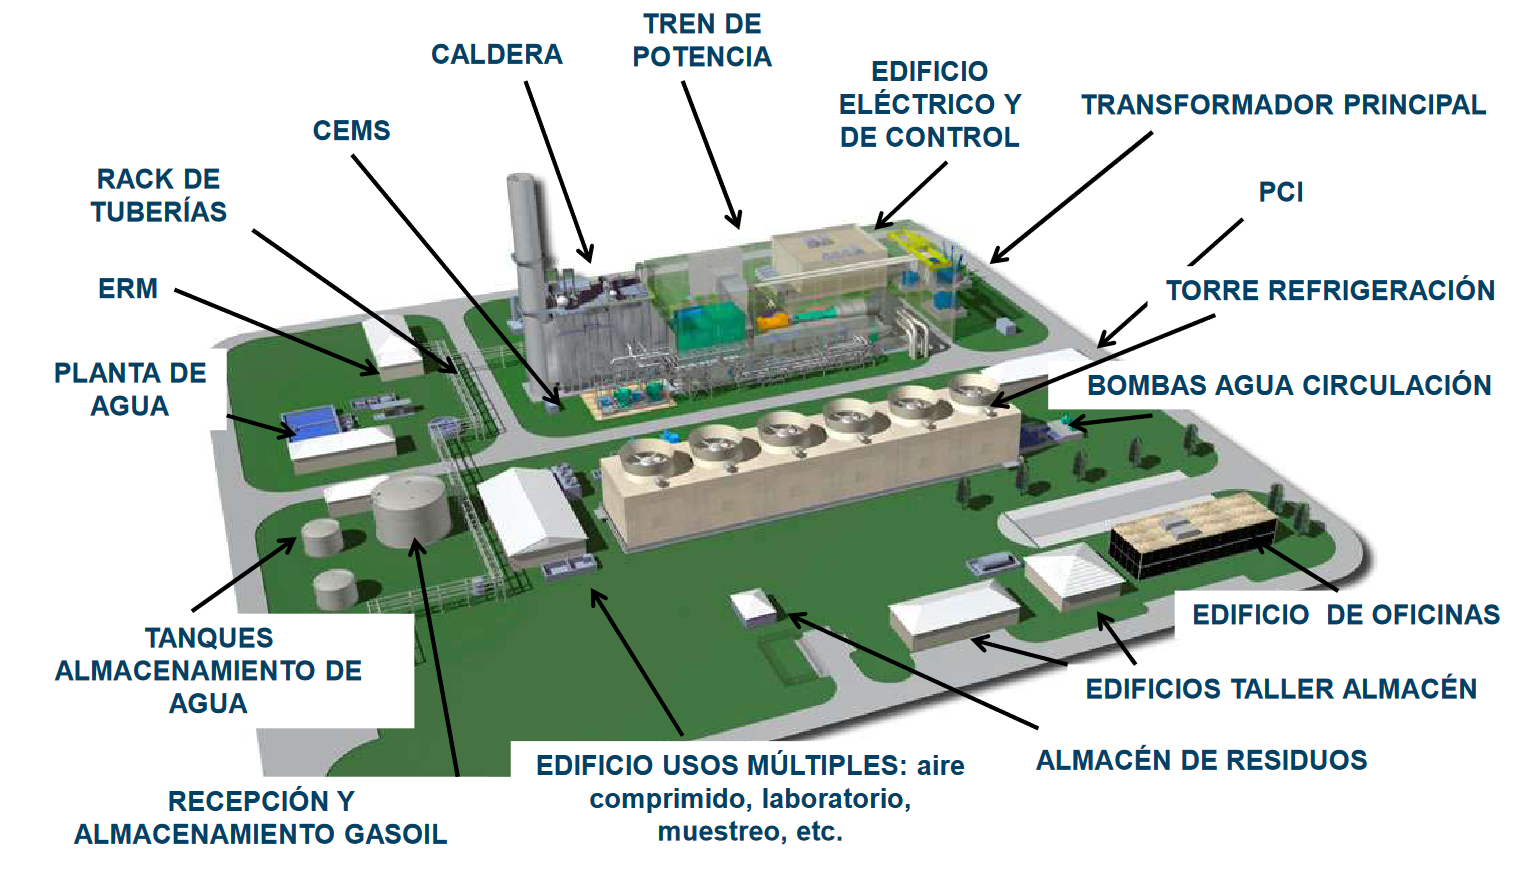
\includegraphics[width=1\linewidth]{res/tema11/partes}
			\label{fig:partes}
		\end{figure}
		
	\section{Ciclo combinado de gas natural.}
		Es la combinación de dos procesos termodinámicos para la producción de energía eléctrica. Un primer proceso consiste en quemar gas en una turbina de gas, y un segundo proceso consiste en aprovechar los gases de escape de la turbina de gas para producir vapor en una caldera de recuperación de calor para finalmente expandirlo en una turbina de vapor.
		\begin{figure}[H]
			\centering
				\begin{circuitikz}[scale = 0.8]
					\tikzstyle{every node}=[font=\footnotesize]
					\draw (13,14) to[L,l={ \footnotesize Economizador} ] (13,16);
					\draw (13,12.25) to[L,l={ \footnotesize Evaporador} ] (13,13.75);
					\draw [ color={rgb,255:red,255; green,0; blue,0}, ](13,10.5) to[L,l={ \footnotesize Sobrecalentador} ] (13,12);
					\draw  (16,14.75) circle (0.75cm) node {\footnotesize Calderín} ;
					\draw [rounded corners = 7.2] (15.5,8.25) rectangle  node {\footnotesize Desgasificador} (18.5,7.25);
					\draw  (7,2.25) circle (1cm) node {\footnotesize Cond.} ;
					\draw [short] (5.5,6.25) -- (5.5,4.25);
					\draw [short] (8.5,5.75) -- (8.5,4.75);
					\draw [short] (8.5,4.75) -- (5.5,4.25);
					\draw [short] (8.5,5.75) -- (5.5,6.25);
					\node [font=\footnotesize] at (7,5.25) {Turbina de vapor};
					\draw [short] (8.25,9.75) -- (8.25,7.75);
					\draw [short] (5.75,9.25) -- (5.75,8.25);
					\draw [short] (8.25,7.75) -- (5.75,8.25);
					\draw [short] (8.25,9.75) -- (5.75,9.25);
					\node [font=\footnotesize] at (7,8.75) {Turbina de gas};
					\draw  (4.25,8.75) circle (0.5cm) node {\footnotesize G} ;
					\draw [dashed] (4.75,8.75) -- (5.75,8.75);
					\draw [->, >=Stealth] (6.5,10.75) -- (6.5,9.5)node[pos=0.35,left]{Aire};
					\draw [->, >=Stealth] (7.5,10.75) -- (7.5,9.75)node[pos=0.5,right]{Combustible};
					\draw [short] (8.25,8.75) -- (13.5,8.75)node[pos=0.5,above]{Flujo calorífico};
					\draw [->, >=Stealth] (13.5,8.75) -- (13.5,18);
					\node [font=\footnotesize] at (13.5,18.25) {Chimenea};
					\draw [short] (13,13.75) -- (16,13.75);
					\draw [short] (16,14) -- (16,13.75);
					\draw [short] (13,14) -- (15.25,14);
					\draw [short] (15.25,14) -- (15.5,14.25);
					\draw [short] (17,7.25) -- (17,6.75);
					\draw [short] (17,6.75) -- (18.75,6.75);
					\draw [short] (18.75,6.75) -- (18.75,16);
					\draw [short] (13,16) -- (18,16);
					\draw [ color={rgb,255:red,255; green,0; blue,0}, short] (13,12.25) -- (17.25,12.25);
					\draw [ color={rgb,255:red,255; green,0; blue,0}, short] (17.25,12.25) -- (17.25,16);
					\draw [ color={rgb,255:red,255; green,0; blue,0}, short] (17.25,16) -- (17.25,16.25);
					\draw [ color={rgb,255:red,255; green,0; blue,0}, short] (17.25,16.25) -- (16,16.25);
					\draw [ color={rgb,255:red,255; green,0; blue,0}, ->, >=Stealth] (16,16.25) -- (16,15.5);
					\draw [ color={rgb,255:red,255; green,0; blue,0}, short] (15.5,15.25) -- (15,15.75);
					\draw [ color={rgb,255:red,255; green,0; blue,0}, short] (15,15.75) -- (14.5,15.75);
					\draw [ color={rgb,255:red,255; green,0; blue,0}, short] (14.5,15.75) -- (14.5,12);
					\draw  (4.25,5.25) circle (0.5cm) node {\footnotesize G} ;
					\draw [dashed] (4.75,5.25) -- (5.5,5.25);
					\draw [ color={rgb,255:red,255; green,0; blue,0}, ->, >=Stealth] (7,6.75) -- (7,6);
					\draw [ color={rgb,255:red,255; green,0; blue,0}, short] (7,6.75) -- (14.5,6.75);
					\draw [ color={rgb,255:red,255; green,0; blue,0}, short] (14.5,6.75) -- (14.5,8);
					\draw [ color={rgb,255:red,255; green,0; blue,0}, short] (14.5,8.25) -- (14.5,8);
					\draw [ color={rgb,255:red,255; green,0; blue,0}, short] (7,4.5) -- (7,4);
					\draw [ color={rgb,255:red,255; green,0; blue,0}, short] (7,4) -- (15,4);
					\draw [ color={rgb,255:red,255; green,0; blue,0}, short] (15,4) -- (15,9);
					\draw [ color={rgb,255:red,255; green,0; blue,0}, short] (15,9) -- (17,9);
					\draw [ color={rgb,255:red,255; green,0; blue,0}, ->, >=Stealth] (17,9) -- (17,8.25);
					\draw [short] (18,16) -- (18.75,16);
					\draw [ color={rgb,255:red,255; green,0; blue,0}, ->, >=Stealth] (7,4) -- (7,3.25);
					\node at (7,4) [circ, color={rgb,255:red,255; green,0; blue,0}] {};
					\draw [short] (8,2.25) -- (16.25,2.25);
					\draw [->, >=Stealth] (16.25,2.25) -- (16.25,7.25);
					\draw [->, >=Stealth] (17,6.75) -- (18,6.75);
					\draw [ color={rgb,255:red,255; green,0; blue,0}, ->, >=Stealth] (15.5,15.25) -- (15.25,15.5);
					\draw [ color={rgb,255:red,255; green,0; blue,0}, ->, >=Stealth] (14.5,15.25) -- (14.5,14.75);
					\draw [ color={rgb,255:red,255; green,0; blue,0}, ->, >=Stealth] (14.5,9.25) -- (14.5,8.5);
					\draw [ color={rgb,255:red,255; green,0; blue,0}, ->, >=Stealth] (12.75,6.75) -- (12,6.75);
					\draw [ color={rgb,255:red,255; green,0; blue,0}, ->, >=Stealth] (9,6.75) -- (8.5,6.75);
					\draw [ color={rgb,255:red,255; green,0; blue,0}, ->, >=Stealth] (8.5,4) -- (8.75,4);
					\draw [ color={rgb,255:red,255; green,0; blue,0}, ->, >=Stealth] (12,4) -- (12.25,4);
					\draw [ color={rgb,255:red,255; green,0; blue,0}, ->, >=Stealth] (15,5.25) -- (15,6);
					\draw [ color={rgb,255:red,255; green,0; blue,0}, ->, >=Stealth] (15.5,9) -- (16.25,9);
					\draw [->, >=Stealth] (18.75,9.5) -- (18.75,10.5);
					\draw [->, >=Stealth] (18.75,13) -- (18.75,13.5);
					\draw [->, >=Stealth] (18.25,16) -- (18,16);
					\draw [ color={rgb,255:red,255; green,0; blue,0}, ->, >=Stealth] (17.25,14.25) -- (17.25,14.5);
					\draw [ color={rgb,255:red,255; green,0; blue,0}, ->, >=Stealth] (15,12.25) -- (15.5,12.25);
					\draw [->, >=Stealth] (15.5,13.75) -- (15,13.75);
					\draw [->, >=Stealth] (13,14) -- (13.5,14);
					\draw [ color={rgb,255:red,255; green,0; blue,0}, short] (14.5,12) -- (13,12);
					\draw [ color={rgb,255:red,255; green,0; blue,0}, short] (13,10.5) -- (14.5,10.5);
					\draw [ color={rgb,255:red,255; green,0; blue,0}, short] (14.5,10.5) -- (14.5,8.25);
					\draw [ color={rgb,255:red,255; green,0; blue,0}, ->, >=Stealth] (13.75,12) -- (13.5,12);
					\draw [ color={rgb,255:red,255; green,0; blue,0}, ->, >=Stealth] (13.5,10.5) -- (13.75,10.5);
					\draw [->, >=Stealth] (9.75,2.25) -- (10.5,2.25);
					\draw [->, >=Stealth] (13.5,2.25) -- (14,2.25);
					\draw [->, >=Stealth] (16.25,4) -- (16.25,4.5);
					\draw [dashed] (8.25,7.75) -- (14.25,7.75);
					\draw [dashed] (14.25,7.75) -- (14.25,16.5);
					\draw [dashed] (14.25,16.5) -- (10,16.5);
					\draw [dashed] (10,16.5) -- (10,9.75);
					\draw [dashed] (8.25,9.75) -- (10,9.75);
				\end{circuitikz}
			\label{fig:my_label}
		\end{figure}
				
		\begin{figure}[H]
			\centering
				\begin{circuitikz}
					\tikzstyle{every node}=[font=\normalsize]
					\draw [->, >=Stealth] (4.5,7) -- (4.5,13);
					\draw [->, >=Stealth] (4.5,7) -- (10.75,7);
					\draw [ color={rgb,255:red,0; green,128; blue,255}, short] (5.5,8.5) .. controls (5.75,9.25) and (6,10) .. (5.75,10.75);
					\draw [ color={rgb,255:red,0; green,128; blue,255}, short] (5.75,10.75) .. controls (7,11) and (7.75,11.5) .. (8.75,13);
					\draw [ color={rgb,255:red,0; green,128; blue,255}, short] (8.75,13) .. controls (9,12) and (9.25,11.75) .. (9.5,11.25);
					\draw [ color={rgb,255:red,0; green,128; blue,255}, short] (9.5,11.25) .. controls (8.25,9.75) and (7.75,9.25) .. (5.5,8.5);
					\draw [ color={rgb,255:red,0; green,0; blue,255}, short] (7,7.5) -- (10.5,7.5);
					\draw [ color={rgb,255:red,0; green,0; blue,255}, short] (10.5,7.5) .. controls (10.25,7.75) and (10,8.25) .. (10,9.5);
					\draw [ color={rgb,255:red,0; green,0; blue,255}, short] (10,9.5) .. controls (10,8.75) and (9.75,8.5) .. (9.5,8.5);
					\draw [ color={rgb,255:red,0; green,0; blue,255}, short] (9.5,8.5) -- (7.75,8.5);
					\draw [ color={rgb,255:red,0; green,0; blue,255}, short] (7.75,8.5) .. controls (7.75,7.75) and (7.5,7.75) .. (7,7.5);
					\node [font=\normalsize, color={rgb,255:red,0; green,128; blue,255}, rotate around={31:(0,0)}] at (7.5,10.5) {Ciclo de gas-aire};
					\node [font=\small, color={rgb,255:red,0; green,0; blue,255}] at (8.9,7.75) {Ciclo agua-vapor};
					\node [font=\normalsize, color={rgb,255:red,0; green,0; blue,255}] at (6.75,7.5) {5};
					\node [font=\normalsize, color={rgb,255:red,0; green,0; blue,255}] at (7.5,8.5) {6};
					\node [font=\normalsize, color={rgb,255:red,0; green,0; blue,255}] at (9.5,8.75) {7};
					\node [font=\normalsize, color={rgb,255:red,0; green,0; blue,255}] at (10,9.75) {8};
					\node [font=\normalsize, color={rgb,255:red,0; green,0; blue,255}] at (10.75,7.5) {9};
					\node [font=\normalsize, color={rgb,255:red,0; green,128; blue,255}] at (5.25,8.5) {1};
					\node [font=\normalsize, color={rgb,255:red,0; green,128; blue,255}] at (5.5,10.75) {2};
					\node [font=\normalsize, color={rgb,255:red,0; green,128; blue,255}] at (8.75,13.25) {3};
					\node [font=\normalsize, color={rgb,255:red,0; green,128; blue,255}] at (9.75,11.25) {4};
					\node [font=\normalsize] at (4.25,13) {T};
					\node [font=\normalsize] at (11,7) {S};
				\end{circuitikz}
			
			\label{fig:my_label}
		\end{figure}
			
	\section{Ciclos de gas.}
		\subsection{Ciclo de Brayton.}
			La turbina de gas puede funcionar como un ciclo abierto, con cámara de combustión, o como un ciclo cerrado con dos intercambiadores de calor.
			\begin{figure}[H]
				\begin{minipage}{0.4\textwidth}
					Compresión y expansión isoentrópicas. El calor se comunica y extrae con $p = cte$.
					
					\vspace{0.25cm}
					El no ser isoentrópico supone bajada del rendimiento $\downarrow\eta \approx 15\%$.
					
					\vspace{0.25cm}
					La potencia del compresor $W_{comp}$ requiere una gran parte de la potencia de la turbina.
					\[W_{comp} \approx 0.2 W_{turb}\]
					
					\vspace{0.25cm}
					Relación de acoplamiento: $\dfrac{W_{comp}}{W_{turb}}$
					
					\vspace{0.25cm}
					Relación de presiones: $r_p = \rho = \dfrac{p_1}{p_2}$
					\[\gamma = 1.4\]
				\end{minipage}
				\begin{minipage}{0.6\textwidth}
					\begin{figure}[H]
						\centering
						\begin{circuitikz}[scale = 0.6]
							\draw [->, >=Stealth] (4,14) -- (4,24.75)node[pos=1,left]{T};
							\draw [->, >=Stealth] (4,14) -- (15.75,14)node[pos=1,below]{S};
							\draw [ color={rgb,255:red,0; green,128; blue,255}, short] (4.75,14.75) -- (4.75,17)node[pos=1,above]{2s};
							\draw [ color={rgb,255:red,0; green,128; blue,255}, short] (4.75,17) .. controls (8.75,19) and (11,20.25) .. (14,24)node[pos=0.5,above]{$p_2$};
							\draw [ color={rgb,255:red,0; green,128; blue,255}, short] (14,24) -- (14,18.75)node[pos=1,below]{4s};
							\draw [ color={rgb,255:red,0; green,128; blue,255}, short] (15.25,19.5) .. controls (11,17) and (9.5,16) .. (4.75,14.75)node[pos=0.5,below]{$p_1$};
							\node at (4.75,14.75) [circ, color={rgb,255:red,0; green,128; blue,255}] {};
							\node at (4.75,17) [circ, color={rgb,255:red,0; green,128; blue,255}] {};
							\node at (14,24) [circ, color={rgb,255:red,0; green,128; blue,255}] {};
							\node at (14,18.75) [circ, color={rgb,255:red,0; green,128; blue,255}] {};
							\node at (5.75,17.5) [circ, color={rgb,255:red,0; green,128; blue,255}] {};
							\node at (15.25,19.5) [circ, color={rgb,255:red,0; green,128; blue,255}] {};
							\draw [ color={rgb,255:red,0; green,128; blue,255}, ->, >=Stealth, dashed] (4.75,14.75) -- (5.25,16.25)node[pos=0,below]{1};
							\draw [ color={rgb,255:red,0; green,128; blue,255}, dashed] (5.25,16.25) -- (5.75,17.5)node[pos=1,above]{2};
							\draw [ color={rgb,255:red,0; green,128; blue,255}, ->, >=Stealth, dashed] (14,24) -- (14.75,21.25)node[pos=0,above]{3};
							\draw [ color={rgb,255:red,0; green,128; blue,255}, dashed] (14.75,21.25) -- (15.25,19.5)node[pos=1,below]{4};
						\end{circuitikz}
						
						\label{fig:my_label}
					\end{figure}
				\end{minipage}
			\end{figure}
			
			
			\begin{figure}[H]
				\begin{minipage}{0.5\textwidth}
					\begin{figure}[H]
						\centering
						\begin{circuitikz}[scale = 0.7]
							\tikzstyle{every node}=[font=\footnotesize]
							\draw [short] (0.75,20.75) -- (0.75,18.75);
							\draw [short] (0.75,18.75) -- (3.25,19.25);
							\draw [short] (0.75,20.75) -- (3.25,20.25);
							\draw [short] (3.25,20.25) -- (3.25,19.25);
							\node [font=\footnotesize] at (2,19.75) {Compresor};
							\node [font=\footnotesize] at (7.5,19.75) {Turbina};
							\draw [short] (8.75,20.75) -- (8.75,18.75);
							\draw [short] (6.25,20.25) -- (8.75,20.75);
							\draw [short] (6.25,19.25) -- (8.75,18.75);
							\draw [short] (6.25,20.25) -- (6.25,19.25);
							\draw  (3,22.25) rectangle  node {\footnotesize Cámara de comb.} (6.5,21.25);
							\draw [->, >=Stealth] (2,21.75) -- (3,21.75);
							\draw [->, >=Stealth] (7.5,21.75) -- (7.5,20.5);
							\draw [short] (2,21.75) -- (2,20.5);
							\draw [short] (6.5,21.75) -- (7.5,21.75);
							\draw [->, >=Stealth] (2,18) -- (2,19)node[pos=0,right]{Aire};
							\draw [->, >=Stealth] (7.5,19) -- (7.5,18)node[pos=1,left]{Gases de escape};
							\draw [dashed] (3.25,19.75) -- (6.25,19.75);
							\draw [dashed] (8.75,19.75) -- (9.75,19.75);
							\draw [->, >=Stealth] (9.5,20.25) .. controls (9.25,20) and (9.25,19.75) .. (9.5,19.25) node[pos=1,below]{W};
							\node [font=\footnotesize] at (1.75,18) {1};
							\node [font=\footnotesize] at (1.75,21.75) {2};
							\node [font=\footnotesize] at (7.75,21.75) {3};
							\node [font=\footnotesize] at (7.75,18) {4};
						\end{circuitikz}
						
						\label{fig:my_label}
						
					\end{figure}
					
					\begin{figure}[H]
						\centering
						\begin{circuitikz}[scale = 0.7]
							\tikzstyle{every node}=[font=\footnotesize]
							\draw [short] (0.75,20.75) -- (0.75,18.75);
							\draw [short] (0.75,18.75) -- (3.25,19.25);
							\draw [short] (0.75,20.75) -- (3.25,20.25);
							\draw [short] (3.25,20.25) -- (3.25,19.25);
							\node [font=\footnotesize] at (2,19.75) {Compresor};
							\node [font=\footnotesize] at (7.5,19.75) {Turbina};
							\draw [short] (8.75,20.75) -- (8.75,18.75);
							\draw [short] (6.25,20.25) -- (8.75,20.75);
							\draw [short] (6.25,19.25) -- (8.75,18.75);
							\draw [short] (6.25,20.25) -- (6.25,19.25);
							\draw  (3,22.25) rectangle  node {\footnotesize Cámara de comb.} (6.5,21.25);
							\draw [->, >=Stealth] (2,21.75) -- (3,21.75);
							\draw [->, >=Stealth] (7.5,21.75) -- (7.5,20.5);
							\draw [short] (2,21.75) -- (2,20.5);
							\draw [short] (6.5,21.75) -- (7.5,21.75);
							\draw [->, >=Stealth] (2,18) -- (2,19);
							\draw [dashed] (3.25,19.75) -- (6.25,19.75);
							\draw [dashed] (8.75,19.75) -- (9.75,19.75);
							\draw [->, >=Stealth] (9.5,20.25) .. controls (9.25,20) and (9.25,19.75) .. (9.5,19.25) node[pos=1,below]{W};
							\node [font=\footnotesize] at (1.75,18) {1};
							\node [font=\footnotesize] at (1.75,21.75) {2};
							\node [font=\footnotesize] at (7.75,21.75) {3};
							\node [font=\footnotesize] at (7.75,18) {4};
							\draw  (3,18.5) rectangle  node {\footnotesize Int. de calor} (6.5,17.5);
							\draw [short] (3,18) -- (2,18);
							\draw [->, >=Stealth] (7.5,18) -- (6.5,18);
							\draw [short] (7.5,18) -- (7.5,19);
							\draw [->, >=Stealth] (4.75,23.25) -- (4.75,22.25)node[pos=0,above]{$\dot Q_e$};
							\draw [->, >=Stealth] (4.75,17.5) -- (4.75,16.5)node[pos=1,below]{$\dot Q_s$};
						\end{circuitikz}
						
						\label{fig:my_label}
					\end{figure}
				\end{minipage}
				\begin{minipage}{0.5\textwidth}
					Suponiendo las capacidades térmicas constantes:
					\[Q_1 = m_{aire}\cdot c_p \cdot (T_3 - T_2)\] \[Q_2 = m_{aire}\cdot c_p \cdot (T_4 - T_1)\]
					
					La expresión del rendimiento resulta:
					\[\eta = 1-\dfrac{Q_2}{Q_1} = 1 - \dfrac{c_p \cdot (T_4 - T_1)}{c_p \cdot (T_3 - T_2)} = 1 - \dfrac{T_1}{T_2} \cdot \dfrac{\dfrac{T_4}{T_1} - 1}{\dfrac{T_3}{T_2} - 1}\]
					
					En las transformaciones adiabáticas:
					\[\left(\dfrac{T_a}{T_b}\right)^\gamma = \left(\dfrac{p_a}{p_b}\right)^{\gamma-1} \Rightarrow \left\{
					\begin{matrix}
						(\text{1-2})\Rightarrow \dfrac{p_2}{p_1} = \left(\dfrac{T_2}{T_1}\right)^{\dfrac{\gamma}{\gamma-1}}\\
						(\text{3-4})\Rightarrow \dfrac{p_3}{p_4} = \left(\dfrac{T_3}{T_4}\right)^{\dfrac{\gamma}{\gamma-1}}
					\end{matrix}
					\right.
					\]
					
					En las transformaciones isobaras:
					\[\left.
					\begin{matrix}
						(\text{2-3})\Rightarrow p_2 = p_3\\
						(\text{4-1})\Rightarrow p_1 = p_4
					\end{matrix}
					\right\}
					\dfrac{p_2}{p_1} = \dfrac{p_3}{p_4}
					\]
					
					Luego el rendimiento resulta:
					\[\eta_{Br} = 1-\dfrac{T_1}{T_2} = 1-\left(\dfrac{p_1}{p_2}\right)^{\dfrac{\gamma}{\gamma-1}} = 1-r_p^{\dfrac{\gamma}{\gamma-1}}\]
				\end{minipage}
			\end{figure}
			
			
			
		\newpage
		\subsection{Ciclo de Brayton regenerativo.}
			El calor cedido al exterior se aprovecha con un intercambiador de calor. Idealmente, a la salida del intercambiador se obtiene la temperatura de salida de los gases de la turbina. Sin embargo se sabe que hay una pérdida de calor y que no se alcanza esta temperatura. Si llamamos $x$ a un punto a la salida del intercambiador e $y$ a la salida de los gases del intercambiador.
			
			\begin{figure}[H]
				\begin{minipage}{0.65\textwidth}
					\begin{figure}[H]
						\centering
						\begin{circuitikz}
							\tikzstyle{every node}=[font=\normalsize]
							\draw [short] (0.75,20.75) -- (0.75,18.75);
							\draw [short] (0.75,18.75) -- (3.25,19.25);
							\draw [short] (0.75,20.75) -- (3.25,20.25);
							\draw [short] (3.25,20.25) -- (3.25,19.25);
							\node [font=\normalsize] at (2,19.75) {Compresor};
							\node [font=\normalsize] at (7.5,19.75) {Turbina};
							\draw [short] (8.75,20.75) -- (8.75,18.75);
							\draw [short] (6.25,20.25) -- (8.75,20.75);
							\draw [short] (6.25,19.25) -- (8.75,18.75);
							\draw [short] (6.25,20.25) -- (6.25,19.25);
							\draw  (4,22.75) rectangle  node {\normalsize Cámara de comb.} (7.5,21.75);
							\draw [->, >=Stealth] (2,20.5) -- (2,23);
							\draw [->, >=Stealth] (6.75,21.75) -- (6.75,20.5);
							\draw [->, >=Stealth] (2,18) -- (2,19);
							\draw [dashed] (3.25,19.75) -- (6.25,19.75);
							\draw [dashed] (8.75,19.75) -- (9.75,19.75);
							\draw [->, >=Stealth] (9.5,20.25) .. controls (9.25,20) and (9.25,19.75) .. (9.5,19.25) node[pos=1,below]{Trabajo};
							\node [font=\normalsize] at (1.75,18) {1};
							\node [font=\normalsize] at (1.75,21.75) {2};
							\node [font=\normalsize] at (7,21) {3};
							\node [font=\normalsize] at (8.5,21.25) {4};
							\draw [short] (8.25,20.75) -- (8.25,21.75);
							\draw [->, >=Stealth] (6.5,23.75) -- (6.5,22.75)node[pos=0,above]{$\dot Q_e$};
							\draw (2.75,24.75) to[L ] (4.25,24.75);
							\draw (4.25,25.75) to[L] (2.75,25.75);
							\node [font=\small] at (3.5,26.25) {Regenerador};
							\draw [, dashed] (2.5,26.5) rectangle  (4.5,24.25);
							\draw [short] (2.75,24.75) -- (2,24.75);
							\draw [short] (2,24.75) -- (2,23);
							\draw [->, >=Stealth] (5,24) -- (5,22.75);
							\draw [short] (4.25,24.75) -- (5,24.75);
							\draw [short] (5,24.75) -- (5,24);
							\draw [->, >=Stealth] (8.25,21.75) -- (8.25,23.75);
							\draw [short] (4.25,25.75) -- (8.25,25.75);
							\draw [short] (8.25,25.75) -- (8.25,23.75);
							\draw [->, >=Stealth] (2.75,25.75) -- (1.25,25.75);
						\end{circuitikz}
						
						\label{fig:my_label}
					\end{figure}
				\end{minipage}
				\begin{minipage}{0.35\textwidth}
					Idealmente:
					\[T_x = T_4 \qquad T_y = T_2\]
					\[Q_1 = m_{aire}c_p(T_3 - T_4)\]
					\[W_{turb} = m_{aire}c_p(T_3 - T_4)\]
					\[W_{comp} = m_{aire}c_p(T_2 - T_1)\]
					
					Luego
					\[Q_1 = W_{turb}\]
					\[\eta = \dfrac{W_{turb} - W_{comp}}{Q_1} = 1-\dfrac{W_{comp}}{W_{turb}} =\]
					\[= 1-\dfrac{T_1}{T_3}\cdot \dfrac{\dfrac{T_2}{T_1} - 1}{1- \dfrac{T_4}{T_3}}\]
					
				\end{minipage}
			\end{figure}
			
			En las transformaciones adiabáticas:
			\[\left(\dfrac{T_a}{T_b}\right)^\gamma = \left(\dfrac{p_a}{p_b}\right)^{\gamma-1} \Rightarrow \left\{
			\begin{matrix}
				(\text{1-2})\Rightarrow \dfrac{p_2}{p_1} = \left(\dfrac{T_2}{T_1}\right)^{\dfrac{\gamma}{\gamma-1}} \Rightarrow \dfrac{T_2}{T_1} = \left(\dfrac{p_2}{p_1}\right)^{\dfrac{\gamma-1}{\gamma}}\\
				(\text{3-4})\Rightarrow \dfrac{p_3}{p_4} = \left(\dfrac{T_3}{T_4}\right)^{\dfrac{\gamma}{\gamma-1}} \Rightarrow \dfrac{T_4}{T_3} = \left(\dfrac{p_3}{p_4}\right)^{\dfrac{\gamma-1}{\gamma}}
			\end{matrix}
			\right.
			\]
			
			En las transformaciones isobaras:
			\[\left.
			\begin{matrix}
				(\text{2-3})\Rightarrow p_2 = p_3\\
				(\text{4-1})\Rightarrow p_1 = p_4
			\end{matrix}
			\right\}
			\dfrac{p_2}{p_1} = \dfrac{p_3}{p_4} \Rightarrow \dfrac{p_4}{p_3} = \dfrac{1}{\dfrac{p_2}{p_1}}
			\]
			
			Luego el rendimiento resulta:
			\[\eta = 1-\dfrac{T_1}{T_3}\cdot \dfrac{\left(\dfrac{p_2}{p_1}\right)^{\dfrac{\gamma-1}{\gamma}} - 1}{1 - \left(\dfrac{p_4}{p_3}\right)^{\dfrac{\gamma-1}{\gamma}}} = 1-\dfrac{T_1}{T_3}\cdot \dfrac{\left(\dfrac{p_2}{p_1}\right)^{\dfrac{\gamma-1}{\gamma}} - 1}{1 - \left(\dfrac{p_1}{p_2}\right)^{\dfrac{\gamma-1}{\gamma}}} = 1-\dfrac{T_1}{T_3}\cdot \dfrac{r_p^{\dfrac{\gamma-1}{\gamma}} - 1}{1 - \left(\dfrac{1}{r_p}\right)^{\dfrac{\gamma-1}{\gamma}}}\]
			
			Y finalmente se llega a la expresión:
			\[\eta_{Br,\,Reg} = 1-\dfrac{T_1}{T_3}\cdot r_p^{\dfrac{\gamma-1}{\gamma}}\]
			\[\uparrow r_p \Rightarrow \downarrow \eta_{Br,\,Reg}\]
			
		
		
		\subsection{Ciclo de Brayton con recalentamiento.}
			\begin{figure}[H]
				\begin{minipage}{0.6\textwidth}
					\begin{figure}[H]
						\centering
						\begin{circuitikz}[scale = 0.6]
							\draw [->, >=Stealth] (4,14) -- (4,24.75)node[pos=1,left]{T};
							\draw [->, >=Stealth] (4,14) -- (15.75,14)node[pos=1,below]{S};
							\draw [ color={rgb,255:red,0; green,128; blue,255}, short] (4.75,14.75) -- (4.75,17)node[pos=1,above]{2};
							\draw [ color={rgb,255:red,0; green,128; blue,255}, short] (4.75,17) .. controls (8.75,19) and (11,20.25) .. (14,24)node[pos=0.5,above]{$p_2$};
							\draw [ color={rgb,255:red,0; green,128; blue,255}, short] (14,24) -- (14,21.25)node[pos=1,left]{a};
							\draw [ color={rgb,255:red,0; green,128; blue,255}, short] (15.25,19.5) .. controls (11,17) and (9.5,16) .. (4.75,14.75)node[pos=0.5,below]{$p_1$};
							\node at (4.75,14.75) [circ, color={rgb,255:red,0; green,128; blue,255}] {};
							\node at (4.75,17) [circ, color={rgb,255:red,0; green,128; blue,255}] {};
							\node at (14,24) [circ, color={rgb,255:red,0; green,128; blue,255}] {};
							\node at (14,18.75) [circ, color={rgb,255:red,0; green,128; blue,255}] {};
							\node at (15.25,19.5) [circ, color={rgb,255:red,0; green,128; blue,255}] {};
							\draw [ color={rgb,255:red,0; green,128; blue,255}, dashed] (14,21.25) -- (14,18.75)node[pos=1,below]{4'};
							\draw [ color={rgb,255:red,0; green,128; blue,255}, short] (14,21.25) .. controls (14.5,21.5) and (14.75,21.5) .. (15.25,22.25)node[pos=0.5,above]{$p_a$};
							\draw [ color={rgb,255:red,0; green,128; blue,255}, short] (15.25,22.25) -- (15.25,19.5)node[pos=1,below]{4};
							\draw [ color={rgb,255:red,0; green,128; blue,255}, ->, >=Stealth] (15.25,21) -- (15.25,20.75);
							\draw [ color={rgb,255:red,0; green,128; blue,255}, short] (14,23.75) -- (14,24);
							\draw [ color={rgb,255:red,0; green,128; blue,255}, short] (14,23.75) -- (14,24)node[pos=1,above]{3};
							\node at (14,21.25) [circ, color={rgb,255:red,0; green,128; blue,255}] {};
							\node at (15.25,22.25) [circ, color={rgb,255:red,0; green,128; blue,255}] {};
							\draw [ color={rgb,255:red,0; green,128; blue,255}, short] (15.25,22) -- (15.25,22.25)node[pos=1,above]{b};
							\draw [ color={rgb,255:red,0; green,128; blue,255}, short] (4.75,15) -- (4.75,14.75)node[pos=1,below]{1};
							\draw [ color={rgb,255:red,255; green,0; blue,0}, ->, >=Stealth] (8,20.25) -- (8.5,19.25)node[pos=0,above]{$Q_{sum}$};
							\draw [ color={rgb,255:red,255; green,0; blue,0}, ->, >=Stealth] (11,16.5) -- (11.5,15.25)node[pos=1,below]{$Q_{ced}$};
							\draw [ color={rgb,255:red,0; green,128; blue,255}, ->, >=Stealth] (4.75,15.75) -- (4.75,16);
							\draw [ color={rgb,255:red,0; green,128; blue,255}, ->, >=Stealth] (14,22.75) -- (14,22.5);
						\end{circuitikz}
						
						\label{fig:my_label}
					\end{figure}
				\end{minipage}
				\begin{minipage}{0.4\textwidth}
					La temperatura máxima viene delimitada por los álabes de la turbina.
					
					\vspace{0.25cm}
					El recalentamiento aumenta el área del ciclo sin aumentar la temperatura máxima.
					
					\vspace{0.25cm}
					La presión intermedia $p_a$ debe hacer que las relaciones de presiones sean iguales:
					\[\dfrac{p_2}{p_a} = \dfrac{p_a}{p_1}\]
				\end{minipage}
			\end{figure}
			
			
			\begin{figure}[H]
				\centering
					\begin{circuitikz}[scale = 0.9]
						\tikzstyle{every node}=[font=\normalsize]
						\draw [short] (0.75,20.75) -- (0.75,18.75);
						\draw [short] (0.75,18.75) -- (3.25,19.25);
						\draw [short] (0.75,20.75) -- (3.25,20.25);
						\draw [short] (3.25,20.25) -- (3.25,19.25);
						\node [font=\normalsize] at (2,19.75) {Compresor};
						\node [font=\normalsize] at (7.5,19.75) {Turbina 1};
						\draw [short] (8.75,20.75) -- (8.75,18.75);
						\draw [short] (6.25,20.25) -- (8.75,20.75);
						\draw [short] (6.25,19.25) -- (8.75,18.75);
						\draw [short] (6.25,20.25) -- (6.25,19.25);
						\draw  (2.75,22.25) rectangle  node {\normalsize Cámara de comb.} (6.25,21.25);
						\draw [->, >=Stealth] (2,21.75) -- (2.75,21.75);
						\draw [->, >=Stealth] (7,21.75) -- (7,20.5);
						\draw [short] (2,21.75) -- (2,20.5);
						\draw [short] (6.25,21.75) -- (7,21.75);
						\draw [dashed] (3.25,19.75) -- (6.25,19.75);
						\draw [dashed] (8.75,19.75) -- (11.75,19.75);
						\draw [->, >=Stealth] (15,20.25) .. controls (14.75,20) and (14.75,19.75) .. (15,19.25) node[pos=1,below]{Trabajo};
						\node [font=\normalsize] at (1.75,18) {1};
						\node [font=\normalsize] at (1.75,21.75) {2};
						\node [font=\normalsize] at (6.75,21.25) {3};
						\node [font=\normalsize] at (13.25,18.5) {4};
						\draw [->, >=Stealth] (4.5,23.25) -- (4.5,22.25)node[pos=0,above]{$\dot Q_{e1}$};
						\draw [short] (8,20.75) -- (8,21.75);
						\node [font=\normalsize] at (13,19.75) {Turbina 2};
						\draw [short] (14.25,20.75) -- (14.25,18.75);
						\draw [short] (11.75,20.25) -- (14.25,20.75);
						\draw [short] (11.75,19.25) -- (14.25,18.75);
						\draw [short] (11.75,20.25) -- (11.75,19.25);
						\draw  (8.75,22.25) rectangle  node {\small C. de recalentamiento} (12.25,21.25);
						\draw [short] (12.25,21.75) -- (13,21.75);
						\draw [->, >=Stealth] (10.5,23.25) -- (10.5,22.25)node[pos=0,above]{$\dot Q_{e2}$};
						\draw [->, >=Stealth] (8,21.75) -- (8.75,21.75);
						\draw [dashed] (14.25,19.75) -- (15.25,19.75);
						\draw [->, >=Stealth] (13,21.75) -- (13,20.5);
						\node [font=\normalsize] at (13.25,21.25) {b};
						\node [font=\normalsize] at (7.75,21.25) {a};
						\draw [->, >=Stealth] (13,19) -- (13,18);
						\draw [->, >=Stealth] (2,18) -- (2,19);
					\end{circuitikz}
				
				\label{fig:my_label}
			\end{figure}
		
		
		\subsection{Ciclo de Brayton con recalentamiento y refrigeración.}
			\begin{figure}[H]
				\begin{minipage}{0.6\textwidth}
					\begin{figure}[H]
						\centering
						\begin{circuitikz}[scale = 0.6]
							\draw [->, >=Stealth] (3,13) -- (3,24.75)node[pos=1,left]{T};
							\draw [->, >=Stealth] (3,13) -- (15.75,13)node[pos=1,below]{S};
							\draw [ color={rgb,255:red,0; green,128; blue,255}, short] (4.75,15.75) -- (4.75,17)node[pos=1,left]{4s};
							\draw [ color={rgb,255:red,0; green,128; blue,255}, short] (4.75,17) .. controls (8.75,19) and (11,20.25) .. (14,24)node[pos=0.5,above]{$p_4$};
							\draw [ color={rgb,255:red,0; green,128; blue,255}, short] (14,24) -- (14,21.25)node[pos=1,left]{7s};
							\draw [ color={rgb,255:red,0; green,128; blue,255}, short] (15.25,19.5) .. controls (10.75,16.75) and (8.75,16) .. (5.75,15)node[pos=0.5,below]{$p_1$};
							\node at (4.75,15.75) [circ, color={rgb,255:red,0; green,128; blue,255}] {};
							\node at (4.75,17) [circ, color={rgb,255:red,0; green,128; blue,255}] {};
							\node at (14,24) [circ, color={rgb,255:red,0; green,128; blue,255}] {};
							\node at (14,18.75) [circ, color={rgb,255:red,0; green,128; blue,255}] {};
							\node at (15.25,19.5) [circ, color={rgb,255:red,0; green,128; blue,255}] {};
							\draw [ color={rgb,255:red,0; green,128; blue,255}, short] (15.25,22.25) -- (15.25,19.5)node[pos=1,below]{9s};
							\draw [ color={rgb,255:red,0; green,128; blue,255}, short] (14,23.75) -- (14,24);
							\draw [ color={rgb,255:red,0; green,128; blue,255}, short] (14,23.75) -- (14,24)node[pos=1,above]{6};
							\node at (14,21.25) [circ, color={rgb,255:red,0; green,128; blue,255}] {};
							\node at (15.25,22.25) [circ, color={rgb,255:red,0; green,128; blue,255}] {};
							\draw [ color={rgb,255:red,0; green,128; blue,255}, short] (15.25,22) -- (15.25,22.25)node[pos=1,above]{8};
							\draw [ color={rgb,255:red,0; green,128; blue,255}, short] (4.75,16) -- (4.75,15.75)node[pos=1,below]{3};
							\draw [ color={rgb,255:red,255; green,0; blue,0}, ->, >=Stealth] (5.25,15.75) -- (5.25,14)node[pos=1,below]{$Q_{ref}$};
							\draw [ color={rgb,255:red,255; green,0; blue,0}, ->, >=Stealth] (14.75,25) -- (14.75,22.75)node[pos=0,above]{$Q_{rec}$};
							\draw [ color={rgb,255:red,0; green,128; blue,255}, short] (14,21.25) -- (15.25,22.25);
							\draw [ color={rgb,255:red,0; green,128; blue,255}, dashed] (5.75,16.25) .. controls (9.25,18) and (12,19.5) .. (15.25,22.25)node[pos=0.5,above]{$p_2$};
							\draw [ color={rgb,255:red,0; green,128; blue,255}, short] (5.75,16.25) -- (5.75,15)node[pos=0,above]{2s};
							\draw [ color={rgb,255:red,0; green,128; blue,255}, short] (5.75,16.25) -- (4.75,15.75);
							\node at (5.75,16.25) [circ, color={rgb,255:red,0; green,128; blue,255}] {};
							\node at (5.75,15) [circ, color={rgb,255:red,0; green,128; blue,255}] {};
							\draw [ color={rgb,255:red,0; green,128; blue,255}, ->, >=Stealth, dashed] (4.75,15.75) -- (5,16.5);
							\draw [ color={rgb,255:red,0; green,128; blue,255}, dashed] (5,16.5) -- (5.25,17.25)node[pos=1,above]{4};
							\node at (5.25,17.25) [circ, color={rgb,255:red,0; green,128; blue,255}] {};
							\draw [ color={rgb,255:red,0; green,128; blue,255}, ->, >=Stealth, dashed] (5.75,15) -- (6,15.75)node[pos=0,below]{1};
							\draw [ color={rgb,255:red,0; green,128; blue,255}, dashed] (6,15.75) -- (6.25,16.5)node[pos=1,above]{2};
							\node at (6.25,16.5) [circ, color={rgb,255:red,0; green,128; blue,255}] {};
							\node at (9.25,19.5) [circ, color={rgb,255:red,0; green,128; blue,255}] {};
							\node [font=\normalsize, color={rgb,255:red,0; green,128; blue,255}] at (9.25,19) {$5$};
							\draw [ color={rgb,255:red,0; green,128; blue,255}, ->, >=Stealth, dashed] (14,24) -- (14.25,22.75);
							\draw [ color={rgb,255:red,0; green,128; blue,255}, dashed] (14.25,22.75) -- (14.5,21.75)node[pos=1,below]{7};
							\node at (14.5,21.75) [circ, color={rgb,255:red,0; green,128; blue,255}] {};
							\node [font=\normalsize, color={rgb,255:red,0; green,128; blue,255}] at (14,18.25) {10};
							\draw [ color={rgb,255:red,0; green,128; blue,255}, dashed] (15.25,19.5) -- (16,20);
							\draw [ color={rgb,255:red,0; green,128; blue,255}, ->, >=Stealth, dashed] (15.25,22.25) -- (15.75,20.75);
							\draw [ color={rgb,255:red,0; green,128; blue,255}, dashed] (15.75,20.75) -- (16,20)node[pos=1,below]{9};
							\node at (16,20) [circ, color={rgb,255:red,0; green,128; blue,255}] {};
							\draw [ color={rgb,255:red,255; green,0; blue,0}, <->, >=Stealth] (7,18) -- (14.5,19.25)node[pos=0.8,above]{$Q_{reg}$};
						\end{circuitikz}
						
						\label{fig:my_label}
					\end{figure}
				\end{minipage}
				\begin{minipage}{0.4\textwidth}
					Para mejorar el funcionamiento se puede introducir una refrigeración intermedia entre dos etapas de compresión, complementando con un recalentamiento y un regenerador. La presión intermedia en el recalentamiento debe ser la misma que en la refrigeración:
					\[\dfrac{p_4}{p_2} = \dfrac{p_2}{p_1}\]
				\end{minipage}
			\end{figure}
			
			\begin{figure}[H]
				\centering
					\begin{circuitikz}[scale=0.6]
						\tikzstyle{every node}=[font=\footnotesize]
						\draw [short] (-1.5,20.75) -- (-1.5,18.75);
						\draw [short] (-1.5,18.75) -- (1,19.25);
						\draw [short] (-1.5,20.75) -- (1,20.25);
						\draw [short] (1,20.25) -- (1,19.25);
						\node [font=\footnotesize] at (-0.25,19.75) {Comp. 2};
						\node [font=\footnotesize] at (7.5,19.75) {Turbina 1};
						\draw [short] (8.75,20.75) -- (8.75,18.75);
						\draw [short] (6.25,20.25) -- (8.75,20.75);
						\draw [short] (6.25,19.25) -- (8.75,18.75);
						\draw [short] (6.25,20.25) -- (6.25,19.25);
						\draw  (2.75,22.25) rectangle  node {\footnotesize C. de comb.} (6.25,21.25);
						\draw [->, >=Stealth] (7,21.75) -- (7,20.5);
						\draw [short] (6.25,21.75) -- (7,21.75);
						\draw [dashed] (1,19.75) -- (6.25,19.75);
						\draw [dashed] (8.75,19.75) -- (12.25,19.75);
						\draw [->, >=Stealth] (15.5,20.25) .. controls (15.25,20) and (15.25,19.75) .. (15.5,19.25) node[pos=1,below]{W};
						\draw [->, >=Stealth] (4.5,23.25) -- (4.5,22.25)node[pos=0,above]{$\dot Q_{e1}$};
						\draw [short] (8,20.75) -- (8,21.75);
						\node [font=\footnotesize] at (13.5,19.75) {Turbina 2};
						\draw [short] (14.75,20.75) -- (14.75,18.75);
						\draw [short] (12.25,20.25) -- (14.75,20.75);
						\draw [short] (12.25,19.25) -- (14.75,18.75);
						\draw [short] (12.25,20.25) -- (12.25,19.25);
						\draw  (8.75,22.25) rectangle  node {\footnotesize C. de recalent.} (12.25,21.25);
						\draw [short] (12.25,21.75) -- (13,21.75);
						\draw [->, >=Stealth] (10.5,23.25) -- (10.5,22.25)node[pos=0,above]{$\dot Q_{e2}$};
						\draw [->, >=Stealth] (8,21.75) -- (8.75,21.75);
						\draw [dashed] (14.75,19.75) -- (15.75,19.75);
						\draw [->, >=Stealth] (13,21.75) -- (13,20.5);
						\draw (0.25,23.5) to[L ] (1.75,23.5);
						\draw (1.75,24.25) to[L] (0.25,24.25);
						\node [font=\footnotesize] at (1,24.75) {Regen.};
						\draw [, dashed] (0,25.25) rectangle  (2,23);
						\draw [short] (1.75,23.5) -- (2.25,23.5);
						\draw [short] (2.25,23.5) -- (2.25,21.75);
						\draw [->, >=Stealth] (2.25,21.75) -- (2.75,21.75);
						\draw [short] (0.25,23.5) -- (-0.25,23.5);
						\draw [short] (-0.25,23.5) -- (-0.25,20.5);
						\draw [short] (1.75,24.25) -- (14,24.25);
						\draw [short] (14,24.25) -- (14,20.75);
						\draw [->, >=Stealth] (-0.25,21.5) -- (-0.25,22);
						\draw [->, >=Stealth] (14,22) -- (14,22.5);
						\draw [->, >=Stealth] (0.25,24.25) -- (-1,24.25);
						\draw (-4.5,17.75) to[L ] (-3,17.75);
						\node [font=\footnotesize] at (-3.75,18.5) {Refrig.};
						\draw [->, >=Stealth] (-3.75,17.25) -- (-3.75,16.25)node[pos=1,below]{$\dot Q_{s}$};
						\draw [short] (-6.75,19) -- (-6.75,17.75);
						\draw [short] (-6.75,17.75) -- (-4.5,17.75);
						\draw [short] (-3,17.75) -- (-0.25,17.75);
						\draw [->, >=Stealth] (-0.25,17.75) -- (-0.25,19);
						\draw [->, >=Stealth] (-7.75,17.75) -- (-7.75,18.75)node[pos=0,below]{Aire};
						\draw [, dashed] (-5,19) rectangle  (-2.5,17.25);
						\node [font=\footnotesize] at (-6.5,18.25) {2};
						\node [font=\footnotesize] at (0,18.25) {3};
						\node [font=\footnotesize] at (-8,18.25) {1};
						\draw [short] (-8.5,20.75) -- (-6,20.25);
						\draw [short] (-6,20.25) -- (-6,19.25);
						\draw [short] (-6,19.25) -- (-8.5,18.75);
						\draw [short] (-8.5,18.75) -- (-8.5,20.75);
						\node [font=\footnotesize] at (-7.25,19.75) {Comp. 1};
						\draw [dashed] (-6,19.75) -- (-1.5,19.75);
						\draw [->, >=Stealth] (-5.75,17.75) -- (-5.5,17.75);
						\node [font=\footnotesize] at (0,21.75) {4};
						\node [font=\footnotesize] at (2,21.75) {5};
						\node [font=\footnotesize] at (6.75,22) {6};
						\node [font=\footnotesize] at (8.25,22) {7};
						\node [font=\footnotesize] at (12.75,22) {8};
						\node [font=\footnotesize] at (14.25,22.5) {9};
						\node [font=\footnotesize] at (-1.5,24.25) {10};
						
					\end{circuitikz}
				
				\label{fig:my_label}
			\end{figure}
		
		\subsection{Compresores.}
			Constructivamente es muy dificil refrigerar un compresor, por lo que se utilizan dos con un refrigerador (ver figura del esquema anterior).
			
			
			El trabajo total es la suma de las dos etapas:
			\[W_{comp} = \dfrac{\gamma R}{\gamma - 1}T_1\left[\left(\dfrac{p_c}{p_1}\right)^{\dfrac{\gamma - 1}{\gamma}}-1\right] + 
			\dfrac{\gamma R}{\gamma - 1}T_2\left[\left(\dfrac{p_2}{p_d}\right)^{\dfrac{\gamma - 1}{\gamma}}-1\right]\]
			
			Donde $p_1$ es la presión en la entrada del primer compresor, $p_2$ la presión a la salida del segundo, $p_c$ la salida del primer compresor y entrada del refrigerador y $p_d$ la salida del refrigerador y entrada del segundo compresor.
			
			
			Idealmente se considera que la temperatura de entrada de la segunda turbina es igual a la de la primera ($T_1 = T_d$), y no se pierde presión en el refrigerador ($p_c = p_d$).
			
	
	\section{Turbinas de gas.}
		Transforman la energía de los gases producidos en la cámara de combustión en energía mecánica, parte de la cual es utilizada por el compresor y auxiliares.
		
		
		Derivan de los motores a reacción de los aviones. Se clasifican según su potencia y tamaño:
		\begin{table}[H]
			\centering
			\begin{tabular}{ccc}
				Tipo & Potencias & Uso\\
				\hline
				Microturbinas		& 30-100 kW & Generación distribuida \\
				Miniturbinas		& 100-500 kW& Emergencia\\
				Turbinas pequeñas	& 1-5 MW	& Cogeneración\\
				Turbinas medianas	& 5-50 MW	& E. Eléctrica de puntas\\
				Turbinas grandes	& 50-300 MW	& E. de base - ciclo combinado
			\end{tabular}
		\end{table}
		
		Partes:
		\begin{itemize}
			\item Conducto de admisión de aire (filtrado).
			\item Enfriador evaporativo.
			\item Compresor rotativo, centrífugo o axial.
			\item Cámara(s) de combustión.
			\item Inyectores.
			\item Cuerpo (radial o axial). Puede ser de alta y baja presión.
			\item Tobera de explusión de gases.
			\item Envolvente.
		\end{itemize}
		
		\subsection{Parámetros característicos.}
			\begin{itemize}
				\item Potencia nominal en condiciones ISO ($T=15\,^\circ C$, $P = 1013\,mbar$, $HR = 60\%$).
				\item Consumo específico de combustible a potencia nominal $[kJ/kWh]$, y referido al PCI del G.N.
				\item Relación de compresión (de 10 a 13 sobre la presión ISO).
				\item Rendimiento.
				\item Caudal másico de aire a potencia nominal, $[kg/s]$ ó $[Nm^3/h]$.
				\item Temperaturas de entrada y salida de los gases a la turbina.
				\item Velocidad de régimen.
				\item Número de quemadores/inyectores.
				\item Caudal másico de gases de escape.
				\item Presión del gas combustible.
				\item Número de cámaras de combustión.
				\item Número de filas de álabes del compresor y de cada uno de los cuerpos de la turbina.
			\end{itemize}
		
		\subsection{Distribución de la energía en la turbina de gas.}
			\begin{figure}[H]
				\centering
					\begin{circuitikz}
						\tikzstyle{every node}=[font=\small]
						\draw [ color={rgb,255:red,0; green,128; blue,255}, short] (-9.5,14.25) -- (-9.5,12.5);
						\draw  (-9.5,15) circle (0.75cm) node {\normalsize C. Comb} ;
						\draw [ color={rgb,255:red,255; green,0; blue,0}, ->, >=Stealth] (-9.5,16.75) -- (-9.5,15.75)node[pos=0,above]{Entrada de calor (100\%)};
						\draw [ color={rgb,255:red,255; green,0; blue,0}, ->, >=Stealth] (-8.75,13) -- (-7.75,13)node[pos=1,right]{Calor expulsado (60\%)};
						\draw [short] (-10.25,13) -- (-10.25,11.75);
						\draw [short] (-10.25,13) -- (-8.75,13.5);
						\draw [short] (-10.25,11.75) -- (-8.75,11.25);
						\draw [short] (-8.75,13.5) -- (-8.75,11.25);
						\draw [short] (-10.25,12.75) -- (-13,12.75);
						\draw [short] (-10.25,12) -- (-13,12);
						\draw [short] (-13,13) -- (-13,11.75);
						\draw [short] (-13,13) -- (-14.5,13.5);
						\draw [short] (-14.5,13.5) -- (-14.5,11.25);
						\draw [short] (-14.5,11.25) -- (-13,11.75);
						\draw [ color={rgb,255:red,255; green,0; blue,0}, short] (-9.5,14.25) -- (-9.5,13);
						\draw [ color={rgb,255:red,255; green,0; blue,0}, short] (-9.5,13) -- (-8.75,13);
						\draw [ color={rgb,255:red,0; green,128; blue,255}, ->, >=Stealth] (-11.5,15) -- (-10.25,15);
						\draw [ color={rgb,255:red,0; green,128; blue,0}, ->, >=Stealth] (-9.5,12.25) -- (-15.5,12.25)node[pos=1,left]{E. Mec. Generador (40\%)};
						\draw [ color={rgb,255:red,0; green,128; blue,255}, short] (-9.5,12.5) -- (-13.75,12.5);
						\draw [ color={rgb,255:red,0; green,128; blue,255}, short] (-13.75,12.5) -- (-13.75,15);
						\draw [ color={rgb,255:red,0; green,128; blue,255}, short] (-13.75,15) -- (-11.5,15);
						\node [font=\small, color={rgb,255:red,0; green,128; blue,255}] at (-12.25,15.25) {E. Mec. Aire Comp. (80\%)};
						\draw [ color={rgb,255:red,0; green,128; blue,0}, ](-9.5,12.5) to[short] (-9.5,12.25);
						\node [font=\small] at (-11.6,11.75) {E. M. Eje (120\%)};
					\end{circuitikz}
				
				\label{fig:my_label}
			\end{figure}
		
		\subsection{Control de las emisiones de NOx.}
			Para controlar las emisiones de los NOx, se inyecta en la cámara de combustión agua o vapor,
			provocando una disminución de la temperatura de los gases de la combustión. 
			
			\subsubsection{Inyección de agua.}
				Se inyecta agua desmineralizada antes de la cámara de combustión. La cantidad de agua que se añade al aire procedente del compresor es la necesaria para que el aire se sature. 
				
				
				La inyección de agua ayuda a bajar la temperatura de entrada del aire en la cámara de combustión y con ello también se ve reducida la temperatura de combustión, ayudando a reducir la producción de NOx. La inyección de agua produce un incremento de la potencia de la turbina gracias al incremento del flujo de masa que pasa a través de la turbina sin tener que incrementar la potencia del compresor.
				
				
				Una turbina de gas con inyección de agua también es conocida como un ciclo evaporativoregenerativo.
				
				\begin{figure}[H]
					\centering
						\begin{circuitikz}
							\tikzstyle{every node}=[font=\normalsize]
							\draw [->, >=Stealth] (-6.75,14) -- (-6.75,15)node[pos=0,below]{Aire};
							\draw [short] (-8,16.75) -- (-5.5,16.25);
							\draw [short] (-5.5,16.25) -- (-5.5,15.25);
							\draw [short] (-5.5,15.25) -- (-8,14.75);
							\draw [short] (-8,14.75) -- (-8,16.75);
							\node [font=\normalsize] at (-6.75,15.75) {Compresor};
							\draw [dashed] (-5.5,15.75) -- (4.5,15.75);
							\draw [->, >=Stealth] (5.75,18.5) -- (5.75,16.5);
							\draw [short] (4.5,15.25) -- (7,14.75);
							\draw [short] (4.5,16.25) -- (4.5,15.25);
							\draw [short] (7,16.75) -- (4.5,16.25);
							\draw [short] (7,14.75) -- (7,16.75);
							\node [font=\normalsize] at (5.75,15.75) {Turbina};
							\draw [dashed] (7,15.75) -- (8,15.75);
							\draw  (-3.75,19.25) rectangle (-2.25,17.75);
							\draw [short] (-3,19.25) -- (-3.5,18.25);
							\draw [short] (-3,19.25) -- (-3.25,18);
							\draw [short] (-3,19.25) -- (-3,18);
							\draw [short] (-3,19.25) -- (-2.75,18);
							\draw [short] (-3,19.25) -- (-2.5,18.25);
							\draw (-0.5,17.75) to[L ] (1,17.75);
							\draw (1,18.5) to[L] (-0.5,18.5);
							\draw (-1.75,14) to[L ] (-1.75,12.5);
							\draw (-1,12.5) to[L ] (-1,14);
							\draw [short] (5.75,15) -- (5.75,14.25);
							\draw [->, >=Stealth] (7.75,16.5) .. controls (7.5,16) and (7.5,15.75) .. (7.75,15) node[pos=1,below]{W};
							\draw  (2.25,19) rectangle  node {\normalsize C. de comb.} (5,18);
							\draw [short] (5.75,18.5) -- (5,18.5);
							\draw [->, >=Stealth] (1,18.5) -- (2.25,18.5);
							\draw [->, >=Stealth] (-2.25,18.5) -- (-0.5,18.5);
							\draw [->, >=Stealth] (-6.75,18.5) -- (-3.75,18.5);
							\draw [short] (-6.75,18.5) -- (-6.75,16.5);
							\draw [, dashed] (-0.75,19.5) rectangle  (1.25,17.25);
							\node [font=\normalsize, rotate around={90:(0,0)}] at (-0.5,13.25) {Precalentador};
							\node [font=\normalsize, rotate around={90:(0,0)}] at (0,13.25) {de agua};
							\draw [, dashed] (-2.25,14.5) rectangle  (0.5,12);
							\draw [->, >=Stealth] (-3,19.75) -- (-3,19.25);
							\draw [short] (-3,19.75) -- (-1.75,19.75);
							\draw [short] (-1.75,19.75) -- (-1.75,14);
							\draw [short] (1,17.75) -- (1.75,17.75);
							\draw [short] (1.75,17.75) -- (1.75,14.25);
							\draw [short] (1.75,14.25) -- (5.75,14.25);
							\draw [short] (-0.5,17.75) -- (-1,17.75);
							\draw [short] (-1,14.75) -- (-1,14);
							\draw [->, >=Stealth] (-1,12.5) -- (-1,11.25)node[pos=1,right]{Salida de gases};
							\draw [->, >=Stealth] (-1.75,11.25) -- (-1.75,11.75)node[pos=0,left]{Entrada de agua};
							\draw [short] (-1.75,12.5) -- (-1.75,11.75);
							\draw [short] (-1,17.75) -- (-1,14.75);
							\draw [->, >=Stealth] (4,14.25) -- (3.75,14.25);
							\draw [->, >=Stealth] (-1,16.5) -- (-1,16.25);
							\node [font=\normalsize, rotate around={-360:(0,0)}] at (-5,19) {C. de inyección};
							\node [font=\normalsize, rotate around={-360:(0,0)}] at (0.25,19) {Regen.};
						\end{circuitikz}
					
					\label{fig:my_label}
				\end{figure}
			
			\subsubsection{Inyección de vapor sobrecalentado.}
				El vapor sobrecalentado procede de un recuperador de calor donde se aprovecha el calor residual de
				los gases de salida de la turbina.
				\begin{figure}[H]
					\centering
						\begin{circuitikz}
							\tikzstyle{every node}=[font=\normalsize]
							\draw [, dashed] (-5.5,14) rectangle  (-2.75,11.5);
							\draw [->, >=Stealth] (-6.75,14) -- (-6.75,15)node[pos=0,below]{Aire};
							\draw [short] (-8,16.75) -- (-5.5,16.25);
							\draw [short] (-5.5,16.25) -- (-5.5,15.25);
							\draw [short] (-5.5,15.25) -- (-8,14.75);
							\draw [short] (-8,14.75) -- (-8,16.75);
							\node [font=\normalsize] at (-6.75,15.75) {Compresor};
							\draw [dashed] (-5.5,15.75) -- (-2.25,15.75);
							\draw [->, >=Stealth] (-1,18.5) -- (-1,16.5);
							\draw [short] (-2.25,15.25) -- (0.25,14.75);
							\draw [short] (-2.25,16.25) -- (-2.25,15.25);
							\draw [short] (0.25,16.75) -- (-2.25,16.25);
							\draw [short] (0.25,14.75) -- (0.25,16.75);
							\node [font=\normalsize] at (-1,15.75) {Turbina};
							\draw [dashed] (0.25,15.75) -- (1.25,15.75);
							\draw (-5,13.5) to[L ] (-5,12);
							\draw (-4.25,12) to[L ] (-4.25,13.5);
							\draw [short] (-1,15) -- (-1,14.5);
							\draw [->, >=Stealth] (1,16.5) .. controls (0.75,16) and (0.75,15.75) .. (1,15) node[pos=1,below]{W};
							\draw  (-4.5,19) rectangle  node {\normalsize C. de comb.} (-1.75,18);
							\draw [short] (-1,18.5) -- (-1.75,18.5);
							\draw [->, >=Stealth] (-6.75,18.5) -- (-4.5,18.5);
							\draw [short] (-6.75,18.5) -- (-6.75,16.5);
							\node [font=\normalsize, rotate around={90:(0,0)}] at (-3.75,12.75) {Recuperador};
							\node [font=\normalsize, rotate around={90:(0,0)}] at (-3.25,12.75) {de calor};
							\draw [short] (-4.25,14.5) -- (-4.25,13.5);
							\draw [->, >=Stealth] (-4.25,12) -- (-4.25,10.75)node[pos=1,right]{Salida de gases};
							\draw [->, >=Stealth] (-5,10.75) -- (-5,11.25)node[pos=0,left]{Entrada de agua};
							\draw [short] (-5,12) -- (-5,11.25);
							\draw [short] (-5,13.5) -- (-5,19.75);
							\draw [short] (-1,14.5) -- (-4.25,14.5);
							\draw [short] (-5,19.75) -- (-3.75,19.75);
							\draw [->, >=Stealth] (-3.75,19.75) -- (-3.75,19);
							\draw [->, >=Stealth] (-2.5,19.75) -- (-2.5,19)node[pos=0,above]{Combustible};
						\end{circuitikz}
					
					\label{fig:my_label}
				\end{figure}			
		
		\subsection{Degradación de la potencia con las horas de funcionamiento.}
			\subsubsection{Lavado con solución detergente.}
				Cada 6000 horas de operación equivalentes se debe lavar el conjunto compresor-turbina en estado de parada. Tras cada lavado se recupera potencia.
				
				
				Cada 1500 horas se realiza un lavado en marcha. Cada 24000 una revisión general.
				
				
				Existen pérdidas de rendimiento no recuperables por el aumento de las pérdidas de rozamiento, tolerancias en los cierres, excentricidades del rotor, etc.
				
				
				Los álabes se corroen si el aire o el combustible contienen vanadio o sodio.
		
		\subsection{Admisión de aire.}
			Su misión es tomar el aire a la presión atmosférica y dirigirlo hacia la boca de entrada del
			compresor.
			\begin{figure}[H]
				\centering
					\begin{circuitikz}[scale = 0.8]
						\tikzstyle{every node}=[font=\footnotesize]
						\draw [->, >=Stealth] (-6.75,14) -- (-6.75,15);
						\draw [short] (-8,16.75) -- (-5.5,16.25);
						\draw [short] (-5.5,16.25) -- (-5.5,15.25);
						\draw [short] (-5.5,15.25) -- (-8,14.75);
						\draw [short] (-8,14.75) -- (-8,16.75);
						\node [font=\footnotesize] at (-6.75,15.75) {Compresor};
						\draw [dashed] (-5.5,15.75) -- (-3,15.75);
						\draw [->, >=Stealth] (-1.75,17.25) -- (-1.75,16.5);
						\draw [short] (-3,15.25) -- (-0.5,14.75);
						\draw [short] (-3,16.25) -- (-3,15.25);
						\draw [short] (-0.5,16.75) -- (-3,16.25);
						\draw [short] (-0.5,14.75) -- (-0.5,16.75);
						\node [font=\footnotesize] at (-1.75,15.75) {Turbina};
						\draw [dashed] (-0.5,15.75) -- (0.5,15.75);
						\draw [short] (-1.75,15) -- (-1.75,14.5);
						\draw [->, >=Stealth] (0.25,16.5) .. controls (0,16) and (0,15.75) .. (0.25,15) node[pos=1,below]{W};
						\draw  (-5.75,17.75) rectangle  node {\footnotesize C. de comb.} (-2.75,16.75);
						\draw [short] (-1.75,17.25) -- (-2.75,17.25);
						\draw [->, >=Stealth] (-6.75,17.25) -- (-5.75,17.25);
						\draw [short] (-6.75,17.25) -- (-6.75,16.5);
						\draw [->, >=Stealth] (-4.25,18.5) -- (-4.25,17.75)node[pos=0,above]{Combustible};
						\draw [, rotate around={-360:(-10.625, 15.75)}] (-11.75,16.75) rectangle (-9.5,14.75);
						\draw [short] (-9.5,16.25) -- (-8.75,16.25);
						\draw [short] (-8.75,16.25) -- (-8.75,14);
						\draw [short] (-8.75,14) -- (-6.75,14);
						\draw [short] (-11.25,16.25) -- (-10,16.25);
						\draw [short] (-11.25,16.25) -- (-12.25,16.25);
						\draw [short] (-12.25,16.25) -- (-12.25,13.75);
						\draw [short] (-11.75,15.25) -- (-9.5,15.25);
						\draw [short] (-10,14.75) -- (-10,13.75);
						\draw  (-11.25,13.75) circle (0.5cm) node {\footnotesize B} ;
						\draw [->, >=Stealth] (-10,13.75) -- (-10.75,13.75);
						\draw [->, >=Stealth] (-12.25,15) -- (-12.25,15.25);
						\draw [short] (-11.75,13.75) -- (-12.25,13.75);
						\draw [short] (-11.25,16.25) -- (-11.5,16);
						\draw [short] (-11.25,16.25) -- (-11,16);
						\draw [short] (-10.5,16.25) -- (-10.75,16);
						\draw [short] (-10.5,16.25) -- (-10.25,16);
						\node [font=\footnotesize, rotate around={-360:(0,0)}] at (-11.25,13) {Bomba de};
						\node [font=\footnotesize, rotate around={-360:(0,0)}] at (-11.25,12.6) {recirculación};
						\draw  (-14.25,17) rectangle (-13.25,14);
						\node [font=\footnotesize, rotate around={90:(0,0)}] at (-13.75,15.5) {Filtro de aire};
						\draw [->, >=Stealth] (-13,15.5) -- (-12.5,15.5);
						\draw [->, >=Stealth] (-15,15.5) -- (-14.5,15.5)node[pos=0,left]{Aire ambiente};
						\draw [->, >=Stealth] (-1.75,14.5) -- (-1.75,14.25);
						\node [font=\footnotesize, rotate around={-360:(0,0)}] at (-10.625,15) {Colector};
						\node [font=\footnotesize] at (-10.625,17.5) {Enfriador};
						\node [font=\footnotesize] at (-10.625,17.1) {evaporativo};
					\end{circuitikz}
				
				\label{fig:my_label}
			\end{figure}
		
		\subsection{Sistema de filtrado de aire.}
			Es necesario filtrar el aire atmosférico para eliminar partículas con un diámetro superior a $5-10\mu m$, que podrían dañar los álabes del compresor. Hay filtros inerciales, de fibra y de superficie autolimpiante.
			
		\subsection{Sistema de enfriamiento de aire. Enfriador evaporativo.}
			La potencia de la turbina de gas y su rendimiento aumentan si se disminuye la temperatura del aire de admisión, ya que de esta manera se incrementa su densidad. Esto se puede lograr mediante un enfriador evaporativo. Al entrar en contacto el aire de admisión no saturado con el agua (en forma de cortina) se produce una evaporación parcial del agua, con el consiguiente enfriamiento del aire y su aumento de densidad.
			
			
			Para evitar el arrastre de gotas de agua, a continuación del enfriador evaporativo se coloca un separador de humedad.
			
			\vspace{0.5cm}
			Características:
			\begin{itemize}
				\item Se usa agua potable.
				\item Se puede enfriar hasta $1\,^\circ C$ por encima de la temperatura del bulbo húmedo.
				\item Baja inversión.
				\item Se produce caída de presión a través de la columna de enfriamiento.
				\item No requiere protección adicional contra la corrosión.
				\item No hay arrastre de gotas hasta la aspiración del compresor.
				\item Aumenta la potencia hasta un 10\%.
				\item Se reduce el consumo específico hasta un 2,5\%.
			\end{itemize}

		\subsection{Compresores.}
			El compresor es la parte de la turbina donde se comprime el fluido de trabajo (aire).
			
			
			El proceso consiste en acelerar el fluido mediante unos alabes móviles para luego llevarlo a una etapa de difusión donde se incrementa la presión, mediante unos alabes fijos. Cada conjunto de alabes móviles más fijos es una etapa del compresor. En la zona de difusión se convierte la energía cinética ganada por el fluido en presión.
			
			
			A medida que se pasa de una etapa a otra el tamaño de los álabes decrece debido al aumento de densidad en el fluido, de forma que se consigue una velocidad axial constante. A medida que aumenta la presión aumenta la temperatura del fluido. 
			
			
			Cuanto mayor sea el incremento de presión en cada etapa mayor será el rendimiento del compresor. El incremento de energía en cada etapa suele ser constante.
		
		
			El aire de una turbina de gas debe entrar a presión. Para ello se utiliza un compresor dinámico. Consta de un rotor, que imparte movimiento a una masa de aire, y un estátor, que transforma la velocidad en presión.
			
			\begin{figure}[H]
				\begin{minipage}{0.6\textwidth}
					\subsubsection{Tipos de conversores dinámicos.}
					\textbf{\textit{Centrífugos:}} hasta un gasto de aire de $40\,kg/s$ y con relaciones de compresión por etapa de 3:1 hasta
					12:1.
					
					\textbf{\textit{Axiales:}} el flujo de aire es paralelo al eje de la máquina. El estátor consta de álabes estacionarios. El conjunto de un rotor y un estator constituye una etapa. El flujo de aire pasa de una etapa a otra y se produce un ligero incremento de presión de 1:1,1 a 1:1,4. Se obtienen relaciones de compresión mayores de 1:15. Los rendimientos que se obtienen son más altos que con los de tipo centrífugo.	
				\end{minipage}
				\begin{minipage}{0.4\textwidth}
					\begin{figure}[H]
						\centering
							\begin{circuitikz}
								\tikzstyle{every node}=[font=\normalsize]
								\draw [->, >=Stealth] (-18.5,11.5) -- (-18.5,15);
								\draw [->, >=Stealth] (-18.5,11.5) -- (-13.75,11.5);
								\draw [ color={rgb,255:red,0; green,128; blue,255}, short] (-18.25,14) -- (-17.5,14);
								\draw [ color={rgb,255:red,0; green,128; blue,255}, short] (-17.5,14) -- (-16.75,14.25);
								\draw [ color={rgb,255:red,0; green,128; blue,255}, short] (-16.75,14.25) -- (-16,14.25);
								\draw [ color={rgb,255:red,0; green,128; blue,255}, short] (-16,14.25) -- (-15.25,14.5);
								\draw [ color={rgb,255:red,0; green,128; blue,255}, short] (-15.25,14.5) -- (-14.5,14.5)node[pos=1,right]{P, T};
								\draw [ color={rgb,255:red,0; green,128; blue,255}, short] (-18.25,12.75) -- (-17.5,12.5);
								\draw [ color={rgb,255:red,0; green,128; blue,255}, short] (-17.5,12.5) -- (-16.75,13.5);
								\draw [ color={rgb,255:red,0; green,128; blue,255}, short] (-16.75,13.5) -- (-16,12.5);
								\draw [ color={rgb,255:red,0; green,128; blue,255}, short] (-16,12.5) -- (-15.25,13.5);
								\draw [ color={rgb,255:red,0; green,128; blue,255}, short] (-15.25,13.5) -- (-14.5,12.5)node[pos=1,right]{V};
								\draw [ color={rgb,255:red,128; green,128; blue,128}, short] (-17.5,15) -- (-17.5,11.75);
								\draw [ color={rgb,255:red,128; green,128; blue,128}, short] (-16,15) -- (-16,11.75);
								\draw [ color={rgb,255:red,128; green,128; blue,128}, short] (-14.5,15) -- (-14.5,11.75);
								\draw [ color={rgb,255:red,128; green,128; blue,128}, dashed] (-16.75,15) -- (-16.75,11.75);
								\draw [ color={rgb,255:red,128; green,128; blue,128}, dashed] (-15.25,15) -- (-15.25,11.75);
								\node [font=\normalsize] at (-16.75,15.25) {Etapa 1};
								\node [font=\normalsize] at (-15.25,15.25) {Etapa 2};
							\end{circuitikz}
						
						\label{fig:my_label}
					\end{figure}
				\end{minipage}
			\end{figure}
			
		\subsection{Cámara de combustión.}
			Es donde se realiza la combustión del gas natural mezclado con el aire a presión que procede del compresor.
			
			
			La relación combustible/aire para una combustión estequiométrica de gas natural es alrededor de 1:15. La relación utilizada en las turbinas de gas suele ser del orden de 1:50 (mayor generación de NOx) para enfriar los gases de la combustión, asegurando una temperatura aceptable a la entrada de la turbina.
		
		\subsection{Turbina de gas. Aspectos constructivos.}
			Existen dos tipos fundamentales:
			\begin{itemize}
				\item \textbf{\textit{Flujo radial.}}
				\item \textbf{\textit{Flujo axial.}} Son las más utilizadas. Los gases circulan paralelos al eje de giro, pasando por las distintas etapas de los álabes.
			\end{itemize}
			
			\subsubsection{Álabes de la turbina de gas.}
				\begin{itemize}
					\item \textbf{\textit{Materiales:}} Se utilizan super-aleaciones a base de níquel en su construcción que permite operan bajo unas condiciones de elevada temperatura y alta presión. Además están recubiertos con renio (Re), un metal raro caracterizado por un punto de fusión muy alto y alta
					densidad. La adición de un 2\% de Re a una mezcla de Co, Ni, Cr, Al e Y	(llamados recubrimientos MCrAlY) le otorga a la mezcla unas propiedades extraordinarias.
					
					\item \textbf{\textit{Refrigeración:}} Las turbinas de gas tienen un circuito interno de aire (proveniente del compresor) que logra una distribución
					uniforme de temperaturas y evita un sobrecalentamiento en los álabes que están expuestos a los gases calientes ($T=1300\,^\circ C$, álabes fijos y móviles de las primeras etapas). 
				\end{itemize}
			
			\subsubsection{Teoría de funcionamiento.}
				En las \textbf{turbinas de impulsión} se produce la caída de entalpía en el álabe fijo, siendo la velocidad circunferencial de entrada a los álabes móviles muy alta. 
				
				
				En las \textbf{turbinas de reacción} la caída de entalpía se produce parte en los álabes fijos y parte en los álabes móviles.
				
				
				Normalmente, las primeras etapas son de impulsión (cero reacción) y las últimas son 50\% de reacción. En esas etapas de impulsión las potencia generada es el doble que en una con un 50\% de reacción, pero sin embargo tienen un rendimiento de menos del 50\%.
				
				
				El incremento en temperaturas de combustión está directamente relacionado con los materiales y la refrigeración en los álabes.
	
	\section{Topología de los ciclos combinados.}
		\begin{figure}[H]
			\centering
				\begin{circuitikz}
					\tikzstyle{every node}=[font=\small]
					\draw  (-11.25,17.75) rectangle  node {\small Ciclo Combinado Gas-Vapor} (-6.75,16.75);
					\draw  (-15,15.75) rectangle  node {\small Sin postcombustión} (-12,15);
					\draw  (-6.25,15.75) rectangle  node {\small Con postcombustión} (-3.25,15);
					\draw  (-7,14) rectangle  node {\small Planta punta} (-5,13.25);
					\draw  (-4.5,14) rectangle  node {\small Planta base} (-2.5,13.25);
					\draw  (-6,12.25) rectangle  node {\small Combustible} (-3.5,11.5);
					\draw  (-9.5,10.5) rectangle  node {\small Mismo combustible (TG/CR)} (-5,9.75);
					\draw  (-4.5,10.5) rectangle  node {\small Distinto combustible (TG/CR)} (0,9.75);
					\draw  (-9.5,8.75) rectangle  node {\small Ciclo de vapor} (-6.5,7.75);
					\draw  (-15.75,6.75) rectangle  node {\small Caldera con 1 nivel de presión} (-11,6);
					\draw  (-10.5,6.75) rectangle  node {\small Caldera con 2 niveles de presión} (-5.5,6);
					\draw [->, >=Stealth] (-10.25,5.5) -- (-9.5,5.5)node[pos=1,right]{Con recalentamiento};
					\draw [->, >=Stealth] (-10.25,5) -- (-9.5,5)node[pos=1,right]{Sin recalentamiento};
					\draw [short] (-10.25,6) -- (-10.25,5);
					\draw  (-5,6.75) rectangle  node {\small Caldera con 3 niveles de presión} (0,6);
					\draw [->, >=Stealth] (-4.75,5.5) -- (-4,5.5)node[pos=1,right]{Con recalentamiento};
					\draw [->, >=Stealth] (-4.75,5) -- (-4,5)node[pos=1,right]{Sin recalentamiento};
					\draw [short] (-4.75,6) -- (-4.75,5);
					\draw [->, >=Stealth] (-8,7.25) -- (-8,6.75);
					\draw [short] (-8,7.75) -- (-8,7.25);
					\draw [short] (-13.5,7.25) -- (-2.5,7.25);
					\draw [->, >=Stealth] (-13.5,7.25) -- (-13.5,6.75);
					\draw [->, >=Stealth] (-2.5,7.25) -- (-2.5,6.75);
					\draw [->, >=Stealth] (-4.75,12.75) -- (-4.75,12.25);
					\draw [short] (-6,13.25) -- (-6,12.75);
					\draw [short] (-6,12.75) -- (-3.5,12.75);
					\draw [short] (-3.5,12.75) -- (-3.5,13.25);
					\draw [->, >=Stealth] (-6,14.5) -- (-6,14);
					\draw [->, >=Stealth] (-3.5,14.5) -- (-3.5,14);
					\draw [short] (-6,14.5) -- (-3.5,14.5);
					\draw [short] (-4.75,11.5) -- (-4.75,11);
					\draw [short] (-7.25,11) -- (-2.25,11);
					\draw [->, >=Stealth] (-7.25,11) -- (-7.25,10.5);
					\draw [->, >=Stealth] (-2.25,11) -- (-2.25,10.5);
					\draw [short] (-4.75,15) -- (-4.75,14.5);
					\draw [->, >=Stealth] (-8,9.25) -- (-8,8.75);
					\draw [short] (-7.25,9.75) -- (-7.25,9.25);
					\draw [short] (-2.25,9.75) -- (-2.25,9.25);
					\draw [short] (-2.25,9.25) -- (-13.5,9.25);
					\draw [short] (-13.5,15) -- (-13.5,9.25);
					\draw [->, >=Stealth] (-13.5,16.25) -- (-13.5,15.75);
					\draw [->, >=Stealth] (-4.75,16.25) -- (-4.75,15.75);
					\draw [short] (-13.5,16.25) -- (-4.75,16.25);
					\draw [short] (-9,16.75) -- (-9,16.25);
				\end{circuitikz}
			
			\label{fig:my_label}
		\end{figure}
		
		\subsection{Tipos de configuración.}
			Se clasifican en función de la configuración de los ejes de la turbina de gas, de vapor y de los generadores.
			\begin{figure}[H]
				\centering
					\begin{circuitikz}
						\tikzstyle{every node}=[font=\normalsize]
						\draw  (-15,13.75) rectangle  node {\normalsize Ciclo combinado} (-12,13);
						\draw [->, >=Stealth] (-14.5,12) -- (-13.75,12)node[pos=1,right]{2TG x 1TV};
						\draw [->, >=Stealth] (-14.5,12.5) -- (-13.75,12.5)node[pos=1,right]{1TG x 1TV};
						\draw [->, >=Stealth] (-11.5,12.25) -- (-10.75,12.25)node[pos=1,right]{Dos ejes};
						\draw [->, >=Stealth] (-11.5,12.75) -- (-10.75,12.75)node[pos=1,right]{Monoeje};
						\draw [->, >=Stealth] (-8.75,13) -- (-8,13)node[pos=1,right]{Embrague síncrono};
						\draw [->, >=Stealth] (-8.75,12.5) -- (-8,12.5)node[pos=1,right]{Acoplamiento rígido};
						\draw [short] (-8.75,13) -- (-8.75,12.5);
						\draw [short] (-14.5,13) -- (-14.5,12);
						\draw [short] (-11.5,12.75) -- (-11.5,12.25);
						\draw [short] (-9.25,12.75) -- (-8.75,12.75);
						\draw [short] (-12,12.5) -- (-11.5,12.5);
					\end{circuitikz}
				
				\label{fig:my_label}
			\end{figure}
			
			\textbf{\textit{Esquema simplificado de un ciclo combinado de dos ejes:}}
			\begin{figure}[H]
				\centering
					\begin{circuitikz}
						\tikzstyle{every node}=[font=\normalsize]
						\draw [short] (-23,9.25) -- (-23,8.25);
						\draw [short] (-23,8.25) -- (-24,7.75);
						\draw [short] (-24,7.75) -- (-24,9.75);
						\draw [short] (-24,9.75) -- (-23,9.25);
						\node [font=\normalsize] at (-23.5,8.75) {C};
						\draw [](-21.25,9.25) to[short] (-21.25,8.25);
						
						\draw [short] (-21.25,8.25) -- (-20.25,7.75);
						\draw [short] (-20.25,7.75) -- (-20.25,9.75);
						\draw [short] (-20.25,9.75) -- (-21.25,9.25);
						\node [font=\normalsize] at (-20.75,8.75) {T};
						\draw [dashed] (-23,8.75) -- (-21.25,8.75);
						\draw [dashed] (-20.25,8.75) -- (-19.5,8.75);
						\draw  (-19,8.75) circle (0.5cm) node {\normalsize G} ;
						\draw  (-23,10.75) rectangle  node {\normalsize C. Comb} (-21.25,9.75);
						\draw [->, >=Stealth] (-23.5,10.25) -- (-23,10.25);
						\draw [->, >=Stealth] (-20.75,10.25) -- (-20.75,9.5);
						\draw [short] (-23.5,10.25) -- (-23.5,9.5);
						\draw [short] (-20.75,10.25) -- (-21.25,10.25);
						\draw [->, >=Stealth] (-23.5,7.25) -- (-23.5,8)node[pos=0,right]{Aire};
						\draw  (-19.25,11.25) rectangle  node {\normalsize Caldera de recuperación} (-14.75,10.25);
						\draw [short] (-20.75,8) -- (-20.75,7.25);
						\draw [short] (-20.75,7.25) -- (-17,7.25);
						\draw [->, >=Stealth] (-17,7.25) -- (-17,10.25);
						\draw [->, >=Stealth] (-17,11.25) -- (-17,12)node[pos=1,right]{Chimenea};
						\draw [](-13.75,11.25) to[short] (-13.75,10.25);
						
						\draw [short] (-13.75,10.25) -- (-12.75,9.75);
						\draw [short] (-12.75,11.75) -- (-13.75,11.25);
						\node [font=\normalsize] at (-13.25,10.75) {T};
						\draw [dashed] (-12.75,10.75) -- (-12,10.75);
						\draw  (-11.5,10.75) circle (0.5cm) node {\normalsize G} ;
						\draw [short] (-12.75,11.75) -- (-12.75,9.75);
						\draw [->, >=Stealth] (-14.75,10.75) -- (-13.75,10.75);
					\end{circuitikz}
				
				\label{fig:my_label}
			\end{figure}
			
			\textbf{\textit{Configuración multieje:}}
			\begin{figure}[H]
				\centering
					\begin{circuitikz}[scale = 0.7]
						\tikzstyle{every node}=[font=\footnotesize]
						\draw [short] (-15.5,10.25) -- (-15.5,9.25);
						\draw [short] (-15.5,9.25) -- (-16.5,8.75);
						\draw [short] (-16.5,8.75) -- (-16.5,10.75);
						\draw [short] (-16.5,10.75) -- (-15.5,10.25);
						\node [font=\footnotesize] at (-16,9.75) {C1};
						\draw  (-15.5,11.75) rectangle  node {\footnotesize C. Comb} (-13.5,10.75);
						\draw [short] (-16,10.5) -- (-16,11.25);
						\draw [->, >=Stealth] (-16,11.25) -- (-15.5,11.25);
						\draw [short] (-13.5,11.25) -- (-13,11.25);
						\draw [->, >=Stealth] (-13,11.25) -- (-13,10.5);
						\draw [dashed] (-15.5,9.75) -- (-13.5,9.75);
						\draw [short] (-13.5,10.25) -- (-13.5,9.25);
						\draw [short] (-13.5,10.25) -- (-12.5,10.75);
						\draw [short] (-13.5,9.25) -- (-12.5,8.75);
						\draw [short] (-12.5,8.75) -- (-12.5,10.75);
						\node [font=\footnotesize] at (-13,9.75) {T1};
						\draw  (-11.25,9.75) circle (0.5cm) node {\footnotesize G1} ;
						\draw [dashed] (-12.5,9.75) -- (-11.75,9.75);
						\draw [->, >=Stealth] (-14.5,12.25) -- (-14.5,11.75)node[pos=0,above]{Combustible};
						\draw [short] (-13,9) -- (-13,8.25);
						\draw [short] (-13,8.25) -- (-10.25,8.25);
						\draw [short] (-10.25,8.25) -- (-10.25,13);
						\draw [short] (-3.25,10.25) -- (-3.25,9.25);
						\draw [short] (-3.25,9.25) -- (-4.25,8.75);
						\draw [short] (-4.25,8.75) -- (-4.25,10.75);
						\draw [short] (-4.25,10.75) -- (-3.25,10.25);
						\node [font=\footnotesize] at (-3.75,9.75) {C2};
						\draw  (-3.25,11.75) rectangle  node {\footnotesize C. Comb} (-1.25,10.75);
						\draw [short] (-3.75,10.5) -- (-3.75,11.25);
						\draw [->, >=Stealth] (-3.75,11.25) -- (-3.25,11.25);
						\draw [short] (-1.25,11.25) -- (-0.75,11.25);
						\draw [->, >=Stealth] (-0.75,11.25) -- (-0.75,10.5);
						\draw [dashed] (-3.25,9.75) -- (-1.25,9.75);
						\draw [short] (-1.25,10.25) -- (-1.25,9.25);
						\draw [short] (-1.25,10.25) -- (-0.25,10.75);
						\draw [short] (-1.25,9.25) -- (-0.25,8.75);
						\draw [short] (-0.25,8.75) -- (-0.25,10.75);
						\node [font=\footnotesize] at (-0.75,9.75) {T2};
						\draw  (1,9.75) circle (0.5cm) node {\footnotesize G2} ;
						\draw [dashed] (-0.25,9.75) -- (0.5,9.75);
						\draw [->, >=Stealth] (-2.25,12.25) -- (-2.25,11.75)node[pos=0,above]{Combustible};
						\draw [short] (-0.75,9) -- (-0.75,8.25);
						\draw [short] (-0.75,8.25) -- (2,8.25);
						\draw [short] (2,8.25) -- (2,13);
						\draw [->, >=Stealth] (-8,11.25) -- (-8,10.5);
						\draw [short] (-8.5,10.25) -- (-8.5,9.25);
						\draw [short] (-8.5,10.25) -- (-7.5,10.75);
						\draw [short] (-8.5,9.25) -- (-7.5,8.75);
						\draw [short] (-7.5,8.75) -- (-7.5,10.75);
						\node [font=\footnotesize] at (-8,9.75) {TV};
						\draw [dashed] (-7.5,9.75) -- (-6.75,9.75);
						\draw [short] (-8,9) -- (-8,8.25);
						\draw  (-6.25,9.75) circle (0.5cm) node {\footnotesize G3} ;
						\draw (-8,8.25) to[L ] (-8,7);
						\draw (-7.25,7) to[L ] (-7.25,8.25);
						\draw [->, >=Stealth] (-7.25,7) -- (-7.25,6.25)node[pos=1,right]{Agua caliente};
						\draw [short] (-7.25,8.25) -- (-7.25,8.5);
						\draw [short] (-7.25,8.5) -- (-6.25,8.5)node[pos=1,right]{Agua};
						\draw [short] (-8,7) -- (-8,6.25);
						\draw [short] (-8,6.25) -- (-9,6.25);
						\draw [short] (-9,6.25) -- (-9,13);
						\draw  (-10.75,14) rectangle (-9.75,13);
						\draw [->, >=Stealth] (-11.75,13.5) -- (-11.75,14.5)node[pos=1,left]{Bypass Chimenea 1};
						\draw [->, >=Stealth] (3.5,13.5) -- (3.5,14.5)node[pos=1,right]{\makecell{Bypass\\Chimenea 2}};
						\draw [short] (-10.75,13.5) -- (-11.75,13.5);
						\draw  (1.5,14) rectangle (2.5,13);
						\draw [short] (2.5,13.5) -- (3.5,13.5);
						\draw  (-10.75,16.75) rectangle (-9.75,15);
						\draw (-10.25,15.25) to[L ] (-10.25,16.5);
						\draw [short] (-10.25,16.5) -- (-9.5,16.5);
						\draw [short] (-10.25,15.25) -- (-9,15.25);
						\draw [short] (-9,13) -- (-9,15.25);
						\draw [->, >=Stealth] (-10.25,14) -- (-10.25,15);
						\draw [->, >=Stealth] (-10.25,16.75) -- (-10.25,17.5)node[pos=1,above]{Chimenea 1};
						\draw  (1.5,16.75) rectangle (2.5,15);
						\draw (2,16.5) to[L ] (2,15.25);
						\draw [short] (1.25,16.5) -- (2,16.5);
						\draw [short] (0.75,15.25) -- (2,15.25);
						\draw [->, >=Stealth] (2,14) -- (2,15);
						\draw [->, >=Stealth] (2,16.75) -- (2,17.5)node[pos=1,above]{Chimenea 2};
						\draw [short] (-9,15.25) -- (0.75,15.25);
						\draw [short] (-8,11.25) -- (-8,15.25);
						\draw [short] (-9,15.25) -- (-9,16.5);
						\draw [short] (-9.5,16.5) -- (1.25,16.5);
						\node at (-9,16.5) [circ] {};
						\node at (-8,15.25) [circ] {};
						\node [font=\footnotesize] at (-4.25,15.5) {Vapor};
						\node [font=\footnotesize] at (-4.25,16.75) {Agua de alimentación de la caldera};
						\draw [->, >=Stealth] (-16,8.25) -- (-16,9)node[pos=0,below]{Aire exterior};
						\draw [->, >=Stealth] (-3.75,8.25) -- (-3.75,9)node[pos=0,below]{Aire exterior};
						\draw [->, >=Stealth] (-6.5,8.5) -- (-6.75,8.5);
						\draw [->, >=Stealth] (-10.25,10.75) -- (-10.25,11);
						\draw [->, >=Stealth] (2,10.75) -- (2,11);
						\draw [->, >=Stealth] (0,16.5) -- (-0.5,16.5);
						\draw [->, >=Stealth] (-7.75,16.5) -- (-8,16.5);
						\draw [->, >=Stealth] (-6.75,15.25) -- (-6.5,15.25);
						\draw [->, >=Stealth] (0.25,15.25) -- (0.75,15.25);
						\node [font=\footnotesize, rotate around={90:(0,0)}] at (-11,16) {Caldera 1};
						\node [font=\footnotesize, rotate around={90:(0,0)}] at (2.75,16) {Caldera 2};
					\end{circuitikz}
				
				\label{fig:my_label}
			\end{figure}
		
		\subsection{Distribución de energía en un ciclo combinado.}
			\begin{figure}[H]
				\centering
					\begin{circuitikz}
						\tikzstyle{every node}=[font=\small]
						\draw [ color={rgb,255:red,255; green,0; blue,0}, ->, >=Stealth] (-9,15.5) -- (-9,14.5)node[pos=0,above]{Energía del combustible};
						\draw  (-9,14) circle (0.5cm);
						\draw [ color={rgb,255:red,255; green,128; blue,0}, ->, >=Stealth] (-9.5,14) -- (-10.5,14);
						\draw [ color={rgb,255:red,255; green,128; blue,0}, ->, >=Stealth] (-8.5,14) -- (-7.5,14);
						\draw [ color={rgb,255:red,255; green,128; blue,0}, ->, >=Stealth] (-9,13.5) -- (-9,12.5);
						\draw  (-9,12) circle (0.5cm);
						\node [font=\small] at (-5.75,13) {Energía en los gases de escape (61.5\%)};
						\node [font=\small] at (-4.5,13.25) {};
						\draw [ color={rgb,255:red,0; green,128; blue,0}, ->, >=Stealth] (-9,11.5) -- (-9,10.5)node[pos=1,left]{Energía por la chimenea (10\%)};
						\draw [ color={rgb,255:red,255; green,128; blue,0}, ->, >=Stealth] (-9.5,12) -- (-10.5,12);
						\draw [ color={rgb,255:red,255; green,128; blue,0}, ->, >=Stealth] (-3.5,12) -- (-2.5,12);
						\draw [ color={rgb,255:red,0; green,128; blue,0}, ->, >=Stealth] (-5.5,11.5) -- (-5.5,10.5)node[pos=1,right]{Energía por el condensador (30\%)};
						\draw [ color={rgb,255:red,255; green,128; blue,0} ] (-7.5,14.5) rectangle (-3.5,13.5);
						\node [font=\small, color={rgb,255:red,255; green,128; blue,0}] at (-11.75,12.25) {Pérdidas por};
						\node [font=\small, color={rgb,255:red,255; green,128; blue,0}] at (-11.75,11.75) {radiación (0,5\%)};
						\node [font=\small, color={rgb,255:red,255; green,128; blue,0}] at (-11.75,14.25) {Pérdidas por};
						\node [font=\small, color={rgb,255:red,255; green,128; blue,0}] at (-11.75,13.75) {radiación (0,5\%)};
						\node [font=\small, color={rgb,255:red,255; green,128; blue,0}] at (-5.5,14.25) {Energía producida por};
						\node [font=\small, color={rgb,255:red,255; green,128; blue,0}] at (-5.5,13.75) {la turbina de gas (38\%)};
						\draw [ color={rgb,255:red,255; green,128; blue,0}, ->, >=Stealth] (-8.5,12) -- (-7.5,12);
						\draw [ color={rgb,255:red,255; green,128; blue,0} ] (-7.5,12.5) rectangle (-3.5,11.5);
						\node [font=\small, color={rgb,255:red,255; green,128; blue,0}] at (-5.5,12.25) {Energía producida por};
						\node [font=\small, color={rgb,255:red,255; green,128; blue,0}] at (-5.5,11.75) {la turbina de vapor (21\%)};
						\node [font=\small, color={rgb,255:red,255; green,128; blue,0}] at (-1.25,12.25) {Pérdidas por};
						\node [font=\small, color={rgb,255:red,255; green,128; blue,0}] at (-1.25,11.75) {radiación (0,2\%)};
					\end{circuitikz}
				
				\label{fig:my_label}
			\end{figure}
		
	\section{Rendimiento del ciclo combinado.}
		Es el trabajo mecánico aprovechable (en la turbina de gas y en la de vapor) entre la energía introducida en la cámara de combustión.
		\[\eta_{cc} = \dfrac{W_{TG} \cdot W_{TV}}{Q_{TG}} = \dfrac{\eta_{TG} Q_{TG} + \eta_{TV} Q_{TV}(1-\eta_{TG})}{Q_{TG}} = \eta_{TG} + \eta_{TV}(1-\eta_{TG})\]
		
		\subsection{Diagramas de intercambio.}
			Describen la variación de energía entre los gases de escape y el agua-vapor de la caldera.
			
			
			Se definen dos puntos de interés:
			\begin{itemize}
				\item \textbf{\textit{Pinch point}}: mínima diferencia de temperaturas entre los gases y el vapor. Su valor influye en el coste de la caldera, puesto que representa la cantidad de área necesaria de intercambio de calor. A más bajo su valor mejor rendimiento en el intercambio de calor. Oscila entre $5$ y $20\,^\circ C$
				
				\item \textbf{\textit{Approach point:}} diferencia entre la temperatura de saturación a la presión de trabajo y la temperatura del agua de salida del economizador. Altas diferencias de temperatura implican mayores choques térmicos.
			\end{itemize}
			
			\subsubsection{Ciclo combinado de un nivel de presión.}
				\begin{figure}[!ht]
					\centering
						\begin{circuitikz}
							\tikzstyle{every node}=[font=\normalsize]
							\draw [->, >=Stealth] (-12.5,10) -- (-12.5,15.75)node[pos=0.5,left]{$T [^\circ C]$};
							\draw [->, >=Stealth] (-12.5,10) -- (-3.25,10)node[pos=0.5,below]{Transferencia de energía [$MW$]};
							\draw [ color={rgb,255:red,0; green,128; blue,255}, ->, >=Stealth] (-9.75,12) -- (-11.25,13);
							\draw [ color={rgb,255:red,0; green,128; blue,255}, short] (-11.25,13) -- (-12.5,13.75);
							\draw [ color={rgb,255:red,0; green,128; blue,255}, short] (-9.75,12) -- (-6.25,12);
							\draw [ color={rgb,255:red,0; green,128; blue,255}, short] (-6.25,12) -- (-6.25,11.75);
							\draw [ color={rgb,255:red,0; green,128; blue,255}, short] (-6.25,11.75) -- (-6,11.75);
							\draw [ color={rgb,255:red,0; green,128; blue,255}, ->, >=Stealth] (-3.75,10) -- (-5,11);
							\draw [ color={rgb,255:red,0; green,128; blue,255}, short] (-5,11) -- (-6,11.75);
							\draw [ color={rgb,255:red,255; green,0; blue,0}, dashed] (-3.75,11.25) -- (-12.5,14.75)node[pos=0.65,above,sloped]{Temperatura de los gases de escape};
							\draw [short] (-6,12) -- (-4.5,12);
							\draw [short] (-6.25,12.25) -- (-4.5,12.25);
							\draw [short] (-4.5,12) -- (-3.75,12);
							\draw [short] (-4.5,12.25) -- (-3.75,12.25);
							\draw [->, >=Stealth] (-4,11.75) -- (-4,12);
							\draw [->, >=Stealth] (-4,12.5) -- (-4,12.25)node[pos=0.5,above]{Pinch point};
							\draw [short] (-6.5,11.75) -- (-7.5,11.75);
							\draw [->, >=Stealth] (-7.25,11.5) -- (-7.25,11.75)node[pos=0.5,below]{Approach point};
							\draw [->, >=Stealth] (-7.25,12.25) -- (-7.25,12);
							\node [font=\normalsize] at (-11.1,15.25) {Sobrecalentador};
							\node [font=\normalsize] at (-7.8,15.25) {Evaporador};
							\node [font=\normalsize] at (-4.5,15.25) {Economizador};
							\draw [ color={rgb,255:red,128; green,128; blue,128}, dashed] (-9.75,15.75) -- (-9.75,10);
							\draw [ color={rgb,255:red,128; green,128; blue,128}, dashed] (-6,15.75) -- (-6,10);
						\end{circuitikz}
					
					\label{fig:my_label}
				\end{figure}
			
			\subsubsection{Ciclo combinado con dos niveles de presión.}
				\begin{figure}[H]
					\centering
						\begin{circuitikz}
							\tikzstyle{every node}=[font=\normalsize]
							\draw [->, >=Stealth] (-12.5,10) -- (-12.5,15.75)node[pos=0.5,left]{$T [^\circ C]$};
							\draw [->, >=Stealth] (-12.5,10) -- (-3.25,10)node[pos=0.5,below]{Transferencia de energía [$MW$]};
							\draw [ color={rgb,255:red,255; green,0; blue,0}, dashed] (-12.5,10.5) -- (-3.5,15.25);
							\draw [ color={rgb,255:red,0; green,128; blue,255}, short] (-12.5,10.25) -- (-10.5,11.25);
							\draw [ color={rgb,255:red,0; green,128; blue,255}, short] (-10.5,11.25) -- (-10.5,11.5);
							\draw [ color={rgb,255:red,0; green,128; blue,255}, short] (-10.5,11.5) -- (-10,11.5);
							\draw [ color={rgb,255:red,0; green,128; blue,255}, short] (-10,11.5) -- (-8.5,12.25);
							\draw [ color={rgb,255:red,0; green,128; blue,255}, short] (-8.5,12.25) -- (-8.5,12.5);
							\draw [ color={rgb,255:red,0; green,128; blue,255}, short] (-8.5,12.5) -- (-5.5,12.5);
							\draw [ color={rgb,255:red,0; green,128; blue,255}, short] (-5.5,12.5) -- (-3.5,14.75);
							\draw [->, >=Stealth] (-9.75,10.25) -- (-11,11)node[pos=0,right]{Econ. BP};
							\draw [->, >=Stealth] (-10.75,12.75) -- (-10.25,11.5)node[pos=0,right]{Evap. BP};
							\draw [->, >=Stealth] (-8.25,11) -- (-9,12)node[pos=0,right]{Econ. AP - Sobre. BP};
							\draw [->, >=Stealth] (-7.5,14) -- (-7,12.5)node[pos=0,left]{Evap. AP};
							\draw [->, >=Stealth] (-5.75,15) -- (-5,13)node[pos=0,left]{Sobre. BP};
						\end{circuitikz}
					
					\label{fig:my_label}
				\end{figure}	
			
		
	\section{Ejemplo de aplicación.}
		Sea una turbina de gas según la siguiente figura:
		\begin{figure}[H]
			\centering
				\begin{circuitikz}[scale = 0.85]
					\tikzstyle{every node}=[font=\normalsize]
					\draw [short] (-15.75,12) -- (-15.75,11);
					\draw [short] (-15.75,11) -- (-16.75,10.5);
					\draw [short] (-16.75,10.5) -- (-16.75,12.5);
					\draw [short] (-16.75,12.5) -- (-15.75,12);
					\draw [short] (-9,12) -- (-9,11);
					\draw [short] (-9,11) -- (-8,10.5);
					\draw [short] (-9,12) -- (-8,12.5);
					\draw [short] (-8,12.5) -- (-8,10.5);
					\draw [short] (-4.5,12) -- (-4.5,11);
					\draw [short] (-4.5,11) -- (-3.5,10.5);
					\draw [short] (-4.5,12) -- (-3.5,12.5);
					\draw [short] (-3.5,12.5) -- (-3.5,10.5);
					\draw  (-11.5,13.25) rectangle  node {\normalsize CC1} (-10,12.25);
					\draw [->, >=Stealth] (-8.5,12.75) -- (-8.5,12.25);
					\draw [short] (-8.5,12.75) -- (-10,12.75);
					\draw [short] (-9.25,13) -- (-9.25,12.5)node[pos=0,above]{5};
					\draw [short] (-11.5,12.75) -- (-13,12.75);
					\draw [short] (-12.25,13) -- (-12.25,12.5)node[pos=0,above]{4};
					\draw [->, >=Stealth] (-11.75,12.75) -- (-11.5,12.75);
					\node [font=\normalsize] at (-16.25,11.5) {C};
					\node [font=\normalsize] at (-8.5,11.5) {$T_{AP}$};
					\node [font=\normalsize] at (-4,11.5) {$T_{BP}$};
					\draw  (-15.25,14.25) rectangle  node {\normalsize Regen.} (-13,12.5);
					\draw [->, >=Stealth] (-3,14) -- (-13,14);
					\draw [->, >=Stealth] (-10.75,14.75) -- (-10.75,13.25)node[pos=0,above]{$F_1 = 0.06$};
					\draw [short] (-4,10.75) -- (-4,10);
					\draw [short] (-4,10) -- (-3,10);
					\draw [short] (-3,10) -- (-3,14);
					\draw [dashed] (-8,11.5) -- (-4.5,11.5);
					\draw [dashed] (-3.5,11.5) -- (-2.5,11.5);
					\draw  (-2,11.5) circle (0.5cm) node {\normalsize G} ;
					\draw  (-6.5,13.25) rectangle  node {\normalsize CC2} (-5,12.25);
					\draw [short] (-8.5,10.75) -- (-8.5,10);
					\draw [short] (-8.5,10) -- (-7.5,10);
					\draw [short] (-7.5,10) -- (-7.5,12.75);
					\draw [->, >=Stealth] (-7.5,12.75) -- (-6.5,12.75);
					\draw [short] (-7,13) -- (-7,12.5)node[pos=0,above]{6};
					\draw [short] (-5,12.75) -- (-4,12.75);
					\draw [->, >=Stealth] (-4,12.75) -- (-4,12.25);
					\draw [short] (-4.5,13) -- (-4.5,12.5)node[pos=0,above]{7};
					\draw [short] (-3.25,12.75) -- (-2.75,12.75)node[pos=1,right]{8};
					\draw [->, >=Stealth] (-5.75,14.75) -- (-5.75,13.25)node[pos=0,above]{$F_2 = 0.05$};
					\draw [->, >=Stealth] (-15.25,14) -- (-17.25,14);
					\draw [->, >=Stealth] (-16.25,12.75) -- (-15.25,12.75);
					\draw [short] (-16.25,12.75) -- (-16.25,12.25);
					\draw  (-18,9.5) rectangle  node {\normalsize Filtro + Evap.} (-14.5,8.5);
					\draw [->, >=Stealth] (-16.25,9.5) -- (-16.25,10.75);
					\draw [->, >=Stealth] (-19,9) -- (-18,9);
					\draw [short] (-18.5,9.25) -- (-18.5,8.75)node[pos=0,above]{1};
					\draw [short] (-16.5,10) -- (-16,10)node[pos=1,right]{2};
					\draw [short] (-15.75,13) -- (-15.75,12.5)node[pos=0,above]{3};
					\draw [short] (-16.75,14.25) -- (-16.75,13.75)node[pos=0,above]{9};
					\node [font=\normalsize] at (-11.75,9.5) {$PCI = 25\,\dfrac{MJ}{Nm^3}$};
					\node [font=\normalsize] at (-11.5,8.5) {2500h de funcionamiento};
					\draw [dashed] (-15.75,11.5) -- (-9,11.5);
				\end{circuitikz}
			
			\label{fig:my_label}
		\end{figure}
		\newpage
		Datos:
		\begin{itemize}
			\item $P_1 = 1\,bar \qquad T_1 = 20\,^\circ C \qquad \dot m_1 = 300\,kg/s$
			\item $T_2 = 10\,^\circ C \qquad T_4 = 433.4\,^\circ C \qquad T_5 = 1000\,^\circ C \qquad T_7 = 900\,^\circ C$
			\item $\rho = r_p = 8$
			\item Presión intermedia = $p_a = 3\,bar$
			\item $\eta_{ISO_C} = 85\% \qquad \eta_{mec_C} = 98\%$
			\item $\eta_{cc1} = \eta_{cc2} = 95\%$
			\item $\eta_{ISO_{BP}} = 98\% \qquad \eta_{ISO_{AP}} = 85\% \qquad \eta_{mec_{TG}} = 98\%$
			\item $\eta_{reg} = 75\% \qquad \eta_{alt} = 85\%$
			\item $c_{p,aire} = 1.0025\,\dfrac{kJ}{kg\cdot K}$
			\item $c_{p,gases} = 1.128\,\dfrac{kJ}{kg\cdot K}$			
		\end{itemize}	
		
		Se pide:
		\begin{enumerate}
			\item Valor de la presión y la temperatura en todos los puntos.
				\begin{figure}[H]
					\centering
						\begin{circuitikz}
							\tikzstyle{every node}=[font=\normalsize]
							\draw [->, >=Stealth] (-14.75,9) -- (-14.75,14.5)node[pos=1,left]{T};
							\draw [->, >=Stealth] (-14.75,9) -- (-8.25,9)node[pos=1,below]{S};
							\draw [ color={rgb,255:red,0; green,128; blue,255}, short] (-14,9.75) -- (-14,11.5);
							\draw [ color={rgb,255:red,0; green,128; blue,255}, short] (-10.25,12.75) -- (-10.25,11.75);
							\draw [ color={rgb,255:red,0; green,128; blue,255}, short] (-9,12.25) -- (-9,11.25);
							\draw [ color={rgb,255:red,0; green,128; blue,255}, short] (-14,11.5) .. controls (-12.75,11.75) and (-11.25,12) .. (-10.25,12.75);
							\draw [ color={rgb,255:red,0; green,128; blue,255}, short] (-10.25,11.75) .. controls (-9.75,11.9) and (-9.5,12) .. (-9,12.25);
							\draw [ color={rgb,255:red,0; green,128; blue,255}, short] (-14,9.75) .. controls (-12.25,10) and (-10.75,10.25) .. (-9,11.25);
							\draw [ color={rgb,255:red,0; green,128; blue,255}, dashed] (-14,9.75) -- (-13,11.75);
							\draw [ color={rgb,255:red,0; green,128; blue,255}, dashed] (-10.25,12.75) -- (-9.5,12);
							\draw [ color={rgb,255:red,0; green,128; blue,255}, dashed] (-9,12.25) -- (-8.5,11.5);
							\draw [ color={rgb,255:red,0; green,128; blue,255}, dashed] (-9,11.25) -- (-8.5,11.5);
							
							
							\node at (-12.5,10) [circ, color={rgb,255:red,0; green,128; blue,255}] 		{};
							\node at (-14,9.75) [circ, color={rgb,255:red,0; green,128; blue,255}] 		{};
							\node at (-14,11.5) [circ, color={rgb,255:red,0; green,128; blue,255}] 		{};
							\node at (-13.025,11.7) [circ, color={rgb,255:red,0; green,128; blue,255}] 	{};
							\node at (-12,11.95) [circ, color={rgb,255:red,0; green,128; blue,255}] 	{};
							\node at (-10.25,12.75) [circ, color={rgb,255:red,0; green,128; blue,255}] 	{};
							\node at (-10.25,11.75) [circ, color={rgb,255:red,0; green,128; blue,255}] 	{};
							\node at (-9.5,12.02) [circ, color={rgb,255:red,0; green,128; blue,255}] 	{};
							\node at (-9,12.25) [circ, color={rgb,255:red,0; green,128; blue,255}] 		{};
							\node at (-8.5,11.5) [circ, color={rgb,255:red,0; green,128; blue,255}] 	{};
							\node at (-9,11.25) [circ, color={rgb,255:red,0; green,128; blue,255}] 		{};
							\node at (-10,10.75) [circ, color={rgb,255:red,0; green,128; blue,255}] 	{};
							
							
							\node [font=\normalsize, color={rgb,255:red,0; green,128; blue,255}] at (-12.5,10.25) {1};
							\node [font=\normalsize, color={rgb,255:red,0; green,128; blue,255}] at (-14,9.5) {2};
							\node [font=\normalsize, color={rgb,255:red,0; green,128; blue,255}] at (-14,11.75) {3s};
							\node [font=\normalsize, color={rgb,255:red,0; green,128; blue,255}] at (-13,12) {3};
							\node [font=\normalsize, color={rgb,255:red,0; green,128; blue,255}] at (-12,12.25) {4};
							\node [font=\normalsize, color={rgb,255:red,0; green,128; blue,255}] at (-10.25,13) {5};
							\node [font=\normalsize, color={rgb,255:red,0; green,128; blue,255}] at (-10.25,11.5) {6s};
							\node [font=\normalsize, color={rgb,255:red,0; green,128; blue,255}] at (-9.5,12.4) {6};
							\node [font=\normalsize, color={rgb,255:red,0; green,128; blue,255}] at (-9,12.5) {7};
							\node [font=\normalsize, color={rgb,255:red,0; green,128; blue,255}] at (-8.25,11.5) {8};
							\node [font=\normalsize, color={rgb,255:red,0; green,128; blue,255}] at (-9,11) {8s};
							\node [font=\normalsize, color={rgb,255:red,0; green,128; blue,255}] at (-10,10.5) {9};
							
						\end{circuitikz}
					
					\label{fig:my_label}
				\end{figure}
				
				Punto 1:
				\[T_1 = 20 + 273.15 = 293.15\,K \qquad P_1 = 1\,bar\]
				
				Punto 2:
				\[T_2 = 10 + 273.15 = 283.15\,K \qquad P_2 = 1\,bar\]
				
				Punto 3:
				\[P_3 = r_p \cdot P_2 = 8\cdot 1 = 8\,bar\]
				\[\dfrac{T_{3s}}{T_2} = \left(\dfrac{P_3}{P_2}\right)^{\dfrac{\gamma - 1}{\gamma}} \Rightarrow T_{3s} = T_2\cdot \left(\dfrac{P_3}{P_2}\right)^{\dfrac{\gamma - 1}{\gamma}} = 512.91\,K\]
				\[\eta_{ISO_C} = \dfrac{T_{3s} - T_2}{T_3 - T_2} \Rightarrow T_3 = T_2 + \dfrac{T_{3s} - T_2}{\eta_{ISO_C}} = 553.45\,K\]
				
				Punto 4:
				\[T_4 = 433.4 + 273.15 = 706.55\,K \qquad P_4 = P_3 = 8\,bar\]
				
				Punto 5:
				\[T_5 = 1000 + 273.15 = 1273.15\,K \qquad P_5 = P_3 = 8\,bar\]
				\newpage
				Punto 6:
				\[P_6 = P_a = 3\,bar\]
				\[\dfrac{T_5}{T_{6s}} = \left(\dfrac{P_5}{P_6}\right)^{\dfrac{\gamma - 1}{\gamma}} \Rightarrow T_{6s} = \dfrac{T_5}{\left(\dfrac{P_3}{P_2}\right)^{\dfrac{\gamma - 1}{\gamma}}} = 961.99\,K\]
				\[\eta_{ISO_{AP}} = \dfrac{T_5 - T_6}{T_5 - T_{6s}} \Rightarrow T_6 = T_5 - \eta_{ISO_{AP}}(T_5 - T_{6s}) = 1008.67\,K\]
				
				Punto 7:
				\[T_7 = 900 + 273.15 = 1173.15\,K \qquad P_7 = P_6 = 3\,bar\]
				
				Punto 8:
				\[P_8 = P_1 = 1\,bar\]
				\[\dfrac{T_7}{T_{8s}} = \left(\dfrac{P_7}{P_8}\right)^{\dfrac{\gamma - 1}{\gamma}} \Rightarrow T_{8s} = \dfrac{T_7}{\left(\dfrac{P_7}{P_8}\right)^{\dfrac{\gamma - 1}{\gamma}}} = 857.1\,K\]
				\[\eta_{ISO_{BP}} = \dfrac{T_7 - T_8}{T_7 - T_{8s}} \Rightarrow T_8 = T_7 - \eta_{ISO_{BP}}(T_7 - T_{8s}) = 863.42\,K\]
				
				Punto 9:
				\[P_9 = P_1 = 1\,bar\]
				\[\eta_{reg} = \dfrac{T_4 - T_3}{T_8 - T_9} \Rightarrow T_9 = T_8 - \dfrac{T_4 - T_3}{\eta_{reg}} = 659.29\,K\]
				
			\item La potencia consumida por el compresor, desarrollada por la turbina y cedida en la cámara de combustión.
			
			
				Compresor:
				\[\dot W_C = h_3 - h_2 = c_{p,\,aire}(T_3 - T_2) = 270.98\,\dfrac{kJ}{kg}\]
				\[W_C = \dot m_1 \cdot \dfrac{\dot W_C}{\eta_{mec_C}} = 300 \cdot \dfrac{270.98}{0.98} = 82.95\,MW\]
				
				Turbina:
				\[\dot W_{TG,\,AP} = h_5 - h_6 = c_{p,\,gases}(T_5 - T_6) = 298.33\,\dfrac{kJ}{kg}\]
				\[W_{TG,\,AP} = \dot m_{1}(1+F_1) \cdot \dot W_{TG,\,AP}\cdot \eta_{mec_{TG}} = 92.97\,MW\]
				
				\[\dot W_{TG,\,BP} = h_7 - h_8 = c_{p,\,gases}(T_7 - T_8) = 349.38\,\dfrac{kJ}{kg}\]
				\[W_{TG,\,BP} = \dot m_{1}(1+F_1+F_2) \cdot \dot W_{TG,\,BP}\cdot \eta_{mec_{TG}} = 114.02\,MW\]
				
				\[W_{TG} = W_{TG,\,AP} + W_{TG,\,BP} = 206.99\,MW\]
				
				Cámaras de combustión:
				\[\dot Q_{cc1} = h_5 - h_4 = c_{p,\,aire}(T_5 - T_4) = 568.02\,\dfrac{kJ}{kg}\]
				\[Q_{cc1} = \dot m_1 (1+F_1)\cdot \dot Q_{cc1} \cdot \eta_{cc1} = 171.60\,MW\]
				
				\[\dot Q_{cc2} = h_7 - h_6 = c_{p,\,gases}(T_7 - T_6) = 185.53\,\dfrac{kJ}{kg}\]
				\[Q_{cc2} = \dot m_1 (1+F_1+F_2)\cdot \dot Q_{cc2} \cdot \eta_{cc2} = 171.60\,MW\]
				
				\[Q_{cc} = Q_{cc1} + Q_{cc2} = 230.29\,MW\]
				
			\item El rendimiento del ciclo, el factor de potencia, el rendimiento eléctrico y la potencia instalada.
				\[\eta_{ciclo} = \dfrac{W_{TG} - W_C}{Q_{cc}} = 53.86\%\]
				\[\varphi_p = 1-\dfrac{W_C}{W_{TG}} = 59.92\%\]
				\[P_{inst} = W_{neto} \cdot \eta_{alt} = (W_{TG} - W_C)\cdot \eta_{alt} = 105.43\,MW\]
				\[\eta_{elec} = \dfrac{P_{inst}}{Q_{cc}} = 45.78\%\]
				
			\item El Heat Rate y el consumo de gas en $\dfrac{Nm^3}{\text{año}}$
				\[HR = \dfrac{Q_{cc}\,\dfrac{kJ}{s}\cdot 3600\,\dfrac{s}{h}}{P_{inst}\,kW} = 7863.51\,\dfrac{kJ}{kWh}\]
				\[Consumo = HR \dfrac{kJ}{kWh}\cdot \dfrac{1\,MJ}{10^3\,kJ}\cdot \dfrac{1\,Nm^3}{25\,MJ} \cdot P_{inst} \cdot Horas/\text{año} = 83.03\,\dfrac{MNm^3}{\text{año}} \]
			
		\end{enumerate}